\chapter{Data measurement}
\label{sec:DataMeasurement}

In this section, we discuss the experimental details involved in measuring $\Lambda$ correlations.
Section \ref{sec:GeneralDetails} covers minutiae about the data sets used in this analysis, the event selection criteria, the relevant subsystems of the ALICE detector, and the code used to perform the analysis.
We describe the process of reconstructing $\Lambda$, including the cuts employed to reduce contamination from secondary or fake $\Lambda$, in Section \ref{sec:ParticleSelection}.
Section \ref{sec:CorrelationFunctionConstruction} details how correlation functions are constructed.
Finally, Section \ref{sec:SysUncertaintyCF} contains a study of the systematic uncertainties on the correlation functions, and plots of the correlation functions with error bars can be found in Section \ref{sec:CorrelationFunctionResults}.

\subsection{General Details}
\label{sec:GeneralDetails}

\subsubsection{Data selection}
\label{sec:DataSelection}

The $\sqrt{s_{NN}}=2.76$ TeV Pb-Pb collision data analyzed in this analysis were recorded at the end of 2011.
This dataset, LHC11h, is comprised of a number of runs.
A "run" refers to the data taken during a continuous recording session of the ALICE detector, as well as to the duration of the recording session.
Runs can include anything from minutes to days of data collection.
Not all runs are used in this analysis.
For example, a particular run might only exist for detector calibration purposes, or a subdetector essential for this analysis might have been offline during data collection.
Runs were selected if they were listed with a Reconstruction Pass 2 global quality of 1 ("Good run") in the ALICE Run Condition Table. 
Approximately 45 million combined central, semi-central and minimum bias events were analyzed. 
The following runs were used:

170593, 170572, 170388, 170387, 170315, 170313, 170312, 170311, 170309, 170308, 170306, 170270, 170269, 170268, 170230, 170228, 170207, 170204, 170203, 170193, 170163, 170159, 170155, 170091, 170089, 170088, 170085, 170084, 170083, 170081, 170040, 170027, 169965, 169923, 169859, 169858, 169855, 169846, 169838, 169837, 169835, 169591, 169590, 169588, 169587, 169586, 169557, 169555, 169554, 169553, 169550, 169515, 169512, 169506, 169504, 169498, 169475, 169420, 169419, 169418, 169417, 169415, 169411, 169238, 169167, 169160, 169156, 169148, 169145, 169144, 169138, 169099, 169094, 169091, 169045, 169044, 169040, 169035, 168992, 168988, 168826, 168777, 168514, 168512, 168511, 168467, 168464, 168460, 168458, 168362, 168361, 168342, 168341, 168325, 168322, 168311, 168310, 168115, 168108, 168107, 168105, 168076, 168069, 167988, 167987, 167985, 167920, 167915

Approximately a third of these runs were taken with the magnetic field of the ALICE detector in the positive configuration, and two-thirds had the magnetic field in the negative configuration.
Having data from both configurations allows for consistency checks; one can see if physics results have any dependence on the detector's magnetic field.

Analysis was also performed on the Monte Carlo HIJING dataset, LHC12a17a\_fix.
The approximately $4.5*10^5$ events in this dataset were reconstructed using calibration information from the following LHC11h runs

170593, 170572, 170388, 170387, 170315, 170313, 170312, 170311, 170309, 170308, 170306, 170270, 170269, 170268, 170230, 170228, 170207, 170204, 170203, 170193, 170163, 170159, 170155, 170091, 170089, 170088, 170085, 170084, 170083, 170081, 170040, 170027, 169965, 169923, 169859, 169858, 169855, 169846, 169838, 169837, 169835

In all cases, the z-component of the primary vertex (the position of the collision within the detector) was required to be within 10 cm of the center of the ALICE detector for an event to be selected.  

\subsubsection{Centrality Flattening}
\label{sec:CentralityFlattening}

Each event is characterized by a centrality percent.
There are 100 centrality bins ranging from 0\%  (head-on collisions) to 99\% (glancing collisions), and the centrality percent is defined such that each bin would be sampled equally using a minimum bias trigger.
The LHC11h dataset employed central and semi-central triggers in addition to the minimum bias trigger, so the centrality bins are not equally filled.
There are approximately as many events in the 0-10\% range as there are in the 10-50\% range.

While the events in the 10-50\% show an even sampling, the number of events in each of the 0-10\% centrality bins differ by a few percent.
This analysis uses a technique called centrality flattening to ensure that each of the 0-10\% bins are sampled evenly.
For each magnetic field configuration, each centrality bin is assigned a weight that brings that bin even with the bin with the smallest overall content (the 9\% bin).
We use those weights and a random number generator to determine whether or not to throw away any given event.

\subsubsection{Detector use}
The data in this analysis utilizes information acquired by several of ALICE's subdetectors.  
Event centrality was measured using the V0 detector with a timing cut from the Zero Degree Calorimeter. 

The neutral $\Lambda$ particle is found by looking for the pion and proton that it decays into.
The Inner Tracking System (ITS), Time Projection Chamber (TPC), Transition Radiation Detector (TRD), and Time of Flight detector (TOF) together provided global particle tracking for these daughter particles.
Information from the TPC is used to perform particle identification (PID), the act of determing if a charged track is a proton, pion, kaon, etc.
%Particle identification (PID) was performed using the TPC, as well as using the Time of Flight detector when possible.


\subsubsection{Analysis code}
The code used in this research to comb through the data, reconstruct $\Lambda$, and measure correlation functions was written in ROOT, an offshoot of C++ designed for statistical analysis and data visualization.
The analysis classes used for this study are checked into the ALICE Collaboration's official code bank, AliPhysics.
The code is stored in the AliPhysics/PWGCF/FEMTOSCOPY/V0LamAnalysis directory, and the classes all have the "AliAnalysisV0Lam" prefix.
The code can be run on the ALICE LEGO (Lightweight Environment for Grid Operators) Train via the macro AliPhysics/PWGCF/FEMTOSCOPY/macros/AddTaskLamLam.C.
The analysis train can run analyses for one or more people simultaneously, thus facilitating efficient usage of resources on the ALICE supercomputing grid.

For this study, the most recent analysis of an ALICE dataset was performed on 06 May, 2016 using AliRoot vAN-20160506-1.
The analysis was run using the Correlations and Fluctuations Physics Working Group (PWGCF) train with dataset LHC11h\_AOD145\_fieldconfigs.

The code used for fitting the measured correlation functions (see Section \ref{sec:FemtoFitter}) is not part of the ALICE code repository.
However, it can be found online at \url{http://github.com/jsalzwedel/FemtoFitting}.
\subsection{Particle selection}
\label{sec:ParticleSelection}


\subsubsection{\texorpdfstring{$\Lambda$}{Lambda} reconstruction}
%\subsubsection{$\Lambda$ reconstruction}
\label{sec:Recon}

$\Lambda$ are neutral particles, and as such we do not directly detect them.  
Instead, $\Lambda$ are topologically reconstructed by looking for the daughter tracks that they decay into.  
The general term for particles reconstructed this way (including $\bar{\Lambda}$ and $K^0_\mathrm{s}$) is V0.

For each event, the list of AliAODv0 objects is used as an initial list of V0 candidates.  
Only AliAODv0 objects with (AliAODv0::GetOnFlyStatus() == false) are used.  
These are V0s constructed offline by the AliV0Vertexer using combined TPC-ITS tracking (or TPC-only if the ITS is inactive).  
After obtaining a list of V0 candidates, the following cuts were applied for each V0's daughter tracks.

\begin{itemize}
\item The V0 was rejected if (AliAODv0::GetNDaughters() $> 2$), and the daughters are required to have different charges.
\item The daughter tracks were required to have hits on at least 80 pad rows of the TPC.
\item The daughter protons and antiprotons were required to have $p_{\rm T} > 0.5$ GeV/$c$, and the daughter pions required $p_{\rm T} \geq 0.16$ GeV/$c$. 
The difference between proton and antiproton $p_{\rm T}$ cuts arises from a need to minimize contaminations from material protons. 
All daughters were required to be in the range $|\eta| < 0.8$.
\item The TPC was used for PID purposes.  
A daughter was considered a proton and/or pion if the PID resolution task returned a respective $\mathrm{d}E/\mathrm{d}x$ NSigma value less than 3 for it.
\item Daughter tracks were required to have a TOF PID NSigma value less than 4 if the TOF signal was available.
\item The proton daughter was required to have a distance of closest approach (DCA) to the primary vertex $> 0.1$ cm.
\item The pion daughter was required to have a DCA to the primary vertex $> 0.3$ cm.
\item The two daughters are required to have a DCA to each other $< 0.4$ cm (the vertex software computes this DCA using resolution weighting, so the units here should probably be called "effective cm").

\end{itemize}

Each V0 is then subjected to the following cuts:
\begin{itemize}
\item The V0 is required to have $|\eta| < 0.8$.
\item The V0 is required to have a proper decay length less than 60 cm.
\item The cosine of the pointing angle must be greater than 0.9993.
\item The DCA of the V0 to the primary vertex must be less than 0.5 cm.
\item For a $\Lambda$ was required to have a proton daughter and a $\pi^-$ daughter (as determined using the above PID cuts).  
For a $\bar{\Lambda}$, an antiproton and $\pi^+$ daughter were required.
\item For both $\Lambda$ and $\bar{\Lambda}$, the reconstructed invariant mass was required to fall within $\abs{m_\mathrm{inv}-m_\mathrm{PDG}} < 3.8$ MeV.  
Note that this cut value was determined by inspection of the $p_\mathrm{T}$-integrated invariant mass peak.  
Future investigation of $p_\mathrm{T}$-dependent invariant mass peak and subsequently enforcing a $p_\mathrm{T}$-dependent cut could lead to better background reduction.  
\end{itemize}

The optimal cut values were determined by comparing distributions of reconstructed $\Lambda$ in Monte Carlo HIJING events with simulated detector effects.  
The data set (LHC12a17a\_fix) included injected strange signals (extra $\Lambda$, $\bar{\Lambda}$, $\Xi$, and $\Omega$ in each event).  
In this analysis, we have estimated the reconstruction efficiency of primary and secondary $\Lambda$ reconstruction efficiency in an effort to account for feeddown effects (see Section \ref{sec:ReconstructionEff}).
The added particles sample a $p_\mathrm{T}$ range that allows for easy detector reconstruction, which skews those efficiency estimates.
Therefore, we have performed our MC analyses with  the injected signals removed.  A primary particle (AliAODMCParticle) was considered injected if it had AliAODMCParticle::GetLabel() greater than AliGenHijingEventHeader::NProduced()$-1$. 
Likewise, a secondary particle (e.g.\ $\Lambda$ resulting from decay of a $\Sigma$ baryon) was considered injected if it's mother particle had AliAODMCParticle::GetLabel() greater than AliGenHijingEventHeader::NProduced()$-1$.  

$\Lambda$ were reconstructed and their corresponding AliAODMCParticle objects were consulted in order to classify the $\Lambda$ into different categories: Real, primary $\Lambda$; secondary $\Lambda$ coming from decays of $\Sigma$ (or $\Sigma$ excited states); secondary $\Lambda$ coming from decays of $\Xi$, $\Omega$, and other sources; fake $\Lambda$; and $K^0_\mathrm{s}$ that have been misidentified as $\Lambda$.  
For each cut parameter (e.g.\ cosine of pointing angle), a plot was made showing the distributions of V0 candidates of the various types.  
These plots contain only the parameter distributions of candidates that pass all the other cuts.  Figures \ref{fig:LambdaCutDists1} and \ref{fig:LambdaCutDists2} show these distributions for the different $\Lambda$ types.  
Figures \ref{fig:AntiLambdaCutDists1} and \ref{fig:AntiLambdaCutDists2} show the equivalent results for $\bar{\Lambda}$.

\begin{figure}
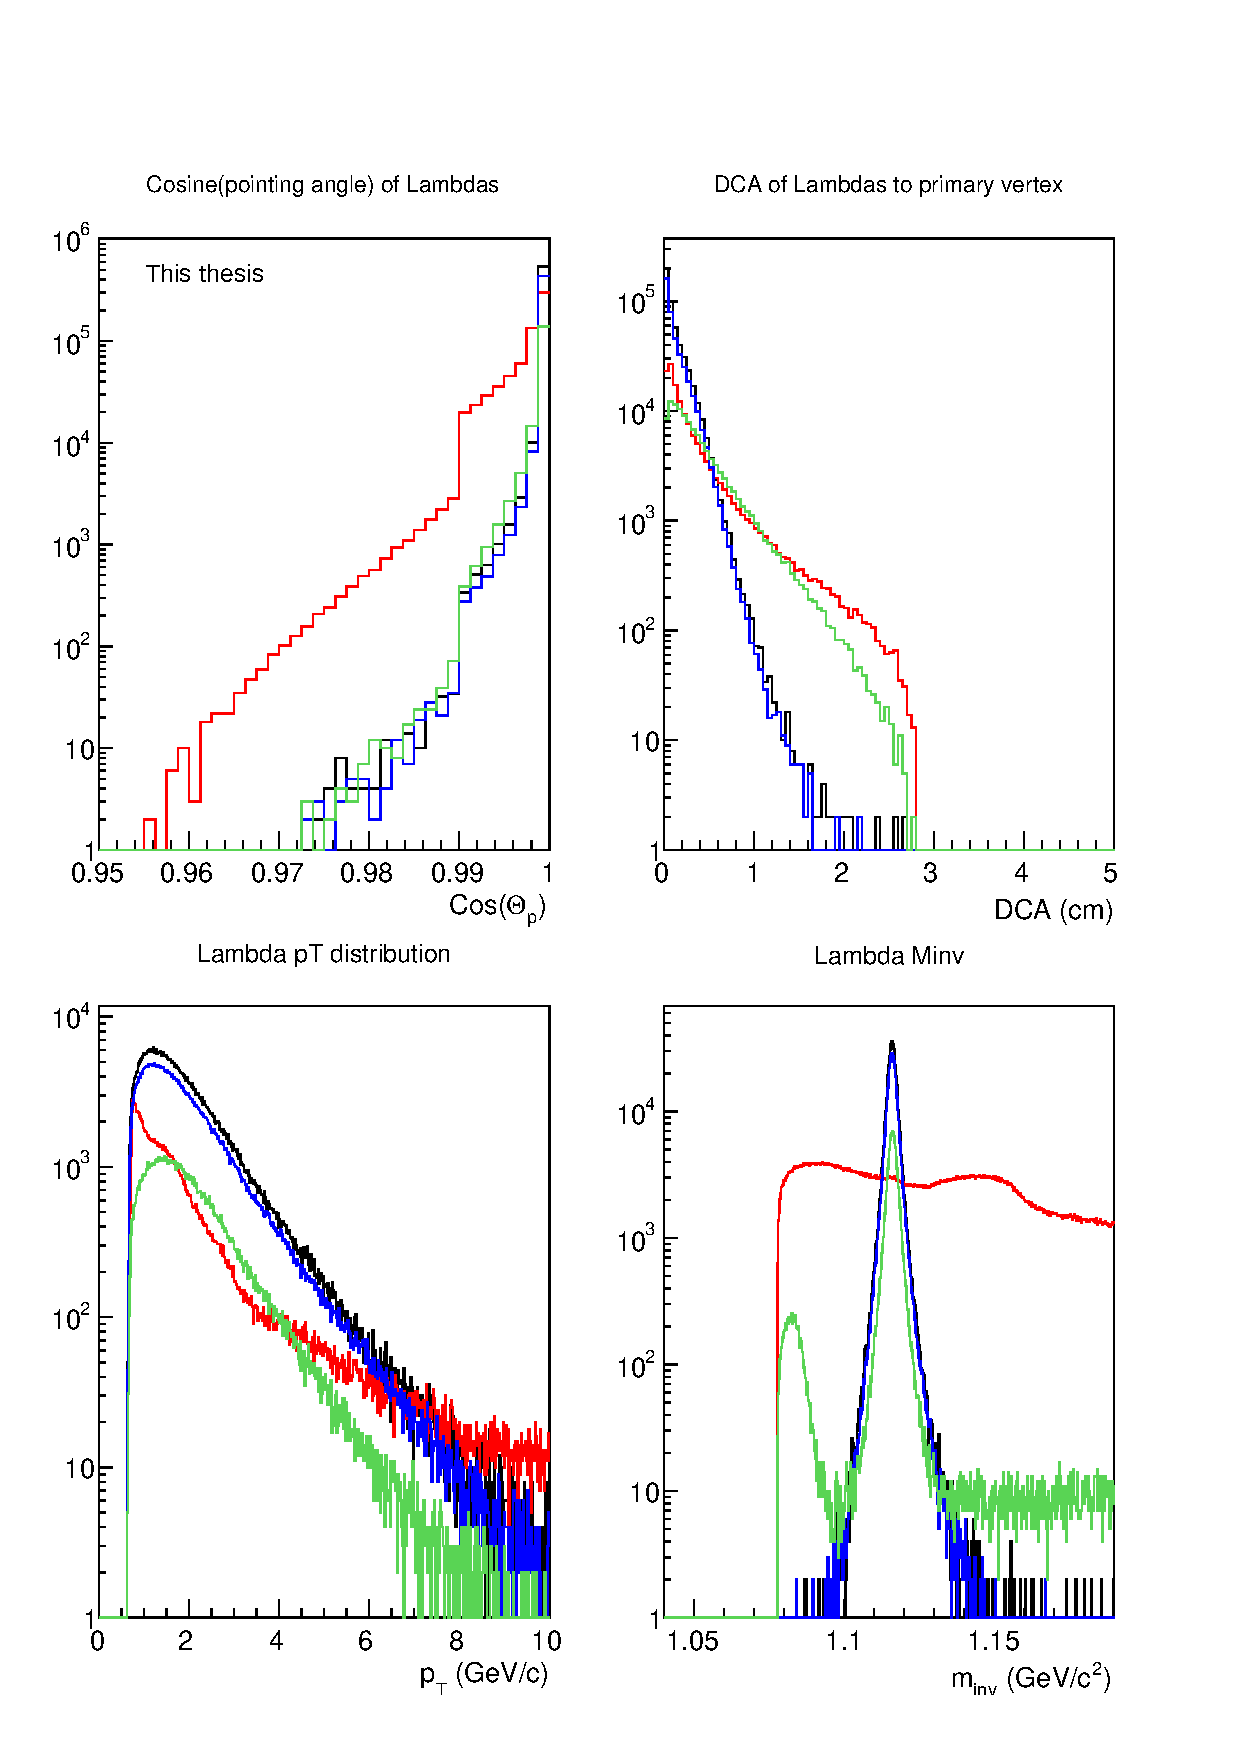
\includegraphics[width=36pc]{Figures/2014-03-31-Distribution-Lambda-4Types-CosP-DCA-pT-Minv.pdf}
\caption[$\Lambda$ cut distributions]{$\Lambda$ cut distributions shown for real $\Lambda$ (black), $\Lambda$ from $\Sigma$ decay (blue), secondary $\Lambda$ from other sources (green), fake $\Lambda$ (red). 
Optimal cut values were set such that a looser cut would differentially add more fake and (non-$\Sigma$) secondary $\Lambda$ than primary $\Lambda$}
\label{fig:LambdaCutDists1}
\end{figure}

\begin{figure}
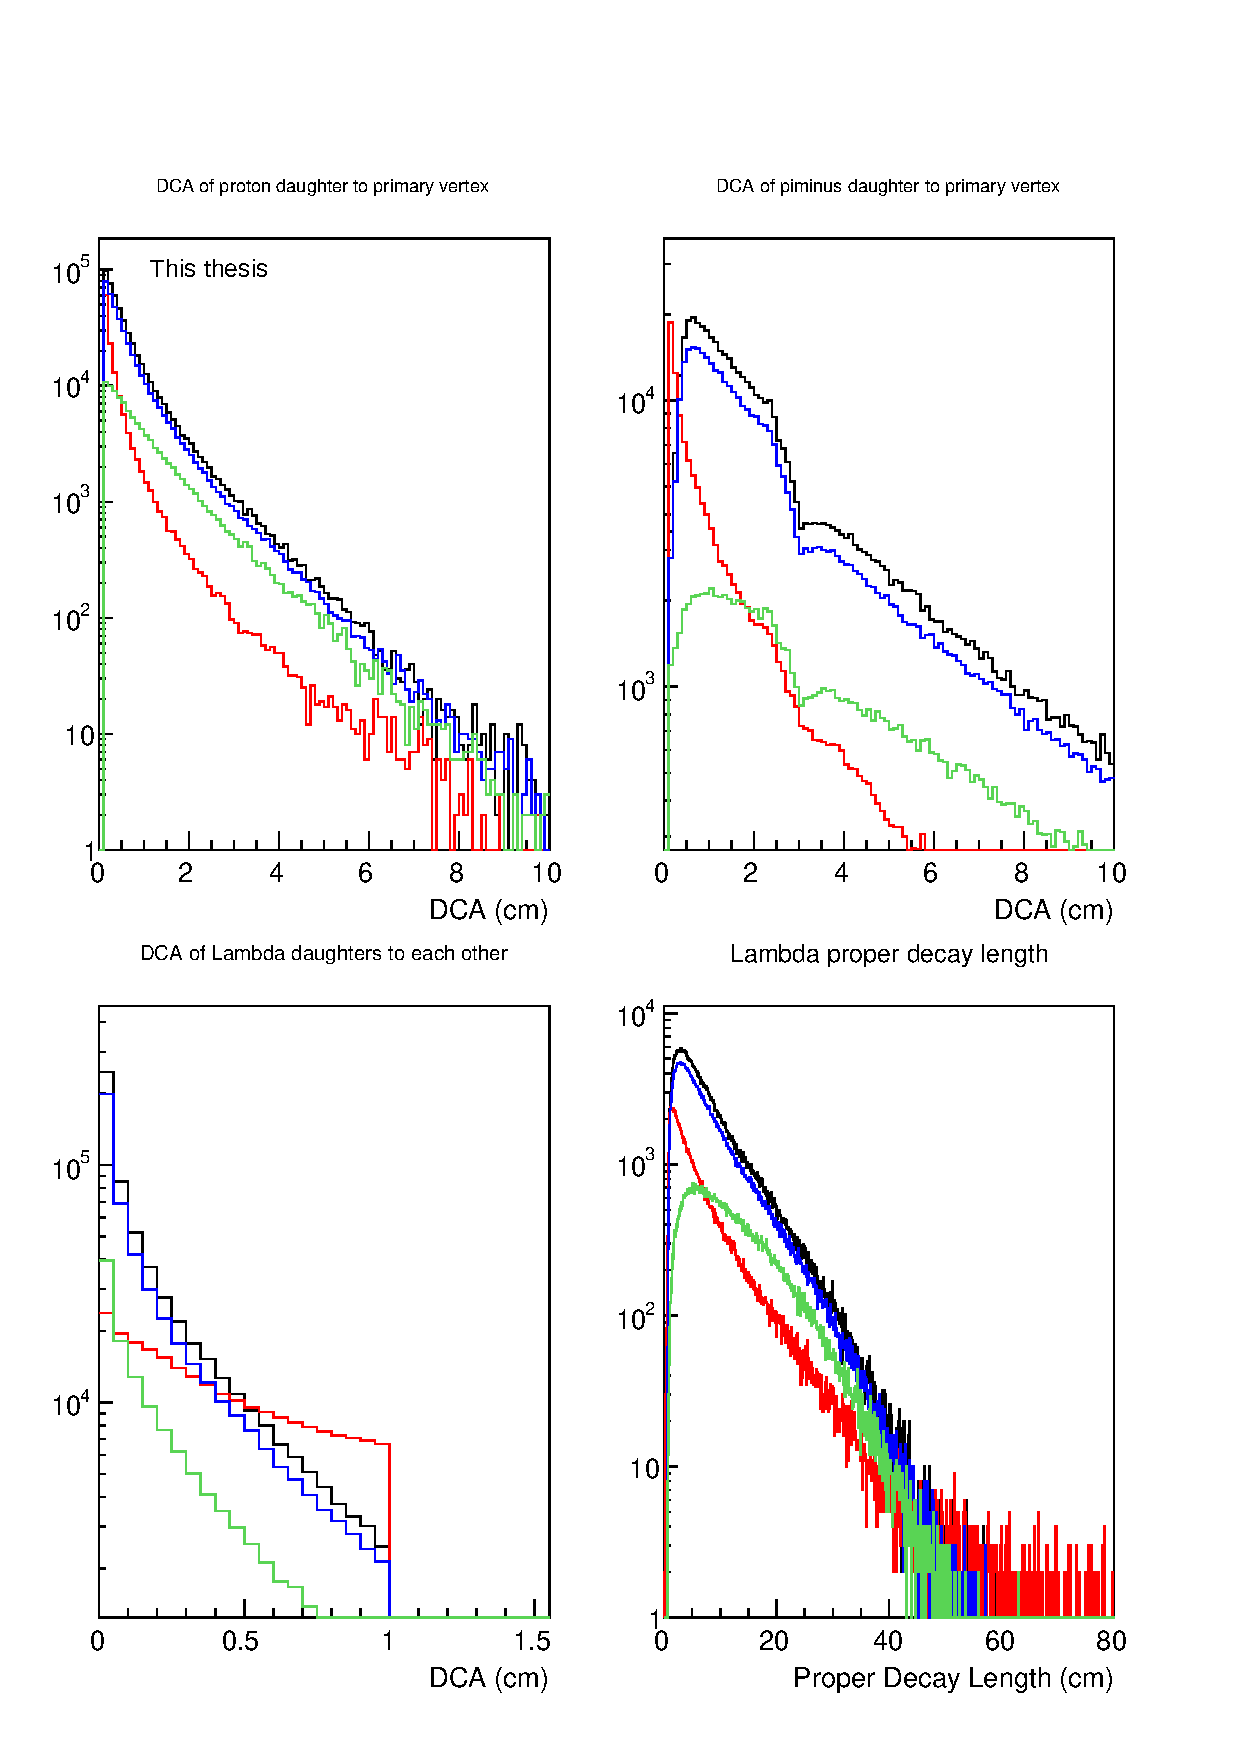
\includegraphics[width=36pc]{Figures/2014-03-31-Distribution-Lambda-4Types-DCA-DCA-DCA-DecayLength.pdf}
\caption[$\Lambda$ cut distributions]{$\Lambda$ cut distributions shown for real $\Lambda$ (black), $\Lambda$ from $\Sigma$ decay (blue), secondary $\Lambda$ from other sources (green), fake $\Lambda$ (red). 
Optimal cut values were set such that a looser cut would differentially add more fake and (non-$\Sigma$) secondary $\Lambda$ than primary $\Lambda$}
\label{fig:LambdaCutDists2}
\end{figure}

\begin{figure}
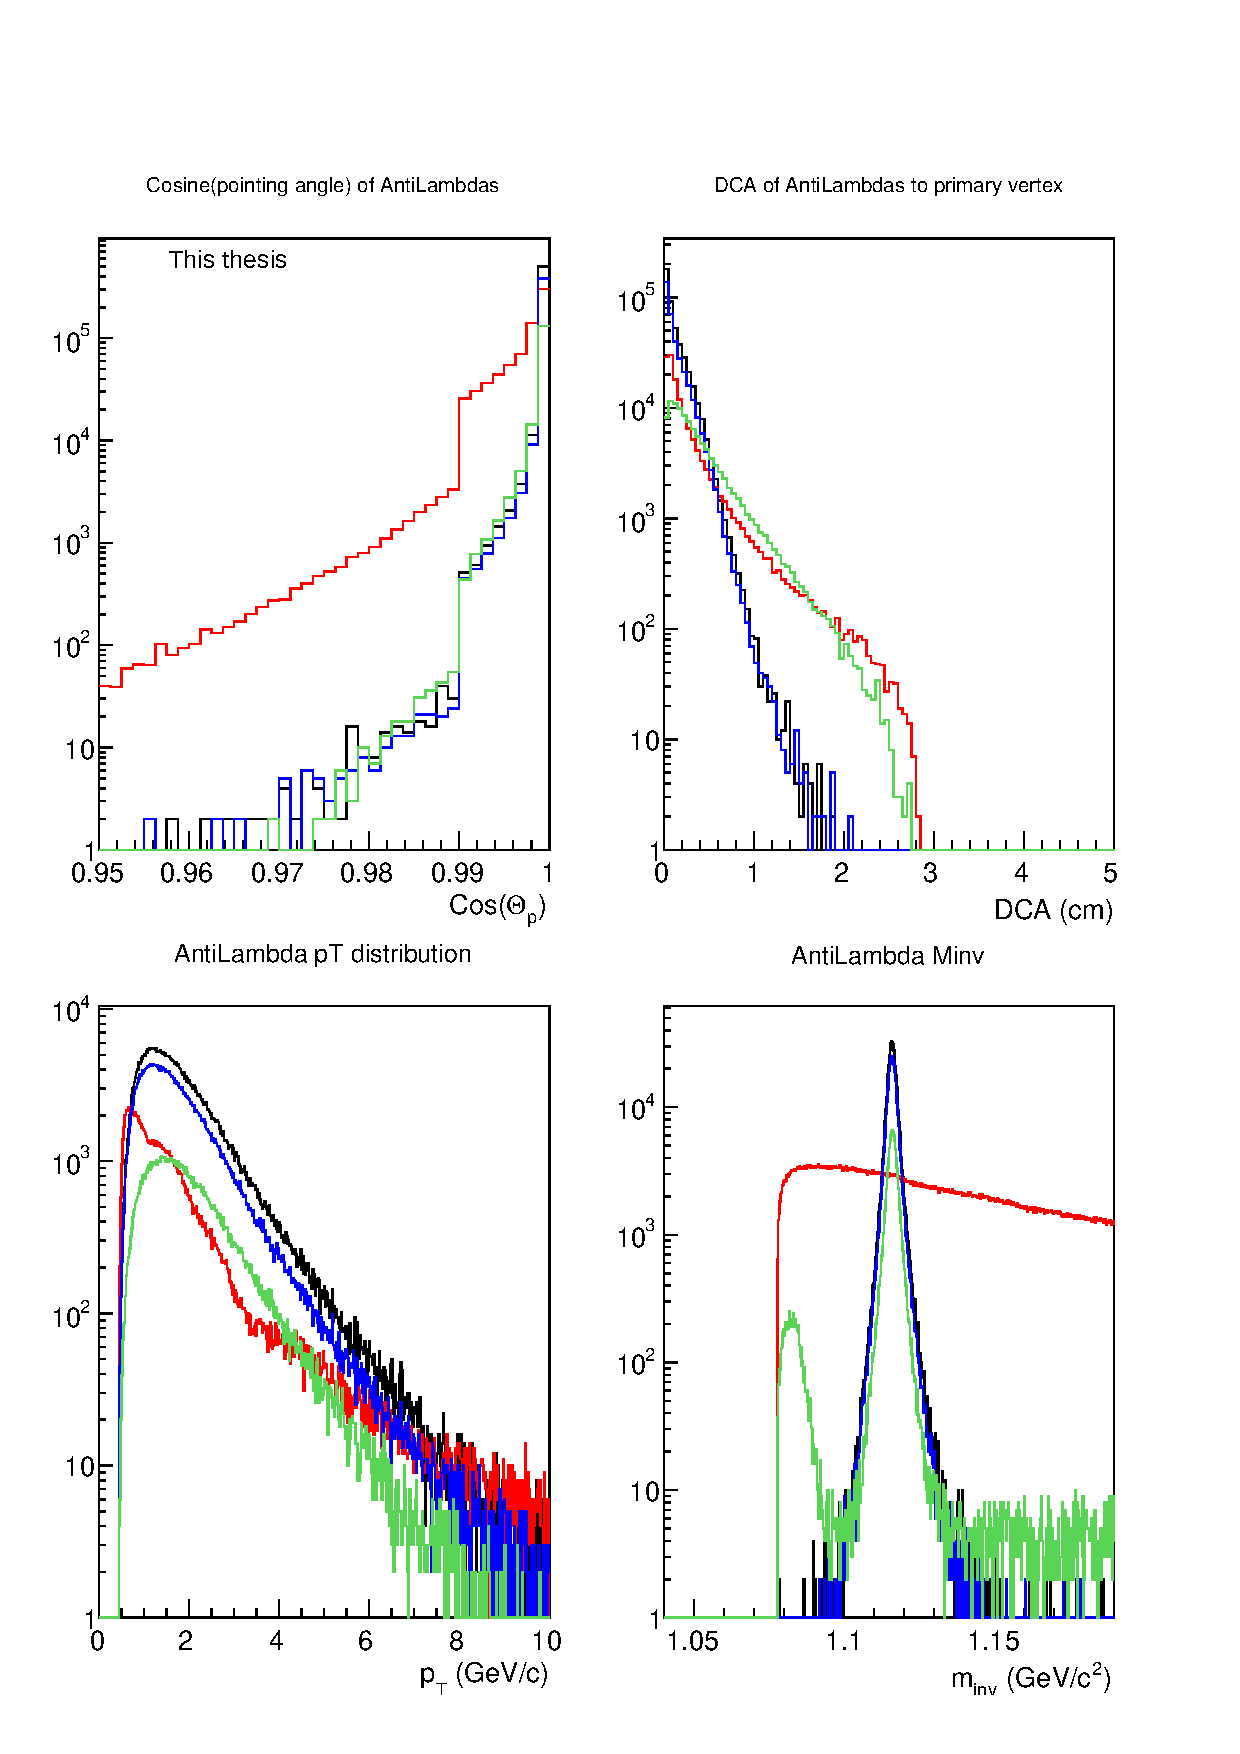
\includegraphics[width=36pc]{Figures/2014-03-31-Distribution-AntiLambda-4Types-CosP-DCA-pT-Minv.pdf}
\caption[$\bar{\Lambda}$ cut distributions]{$\bar{\Lambda}$ cut distributions shown for real $\bar{\Lambda}$ (black), $\bar{\Lambda}$ from $\Sigma$ decay (blue), secondary $\bar{\Lambda}$ from other sources (green), fake $\bar{\Lambda}$ (red). 
Optimal cut values were set such that a looser cut would differentially add more fake and (non-$\bar{\Sigma}$) secondary $\bar{\Lambda}$ than primary $\bar{\Lambda}$}
\label{fig:AntiLambdaCutDists1}
\end{figure}

\begin{figure}
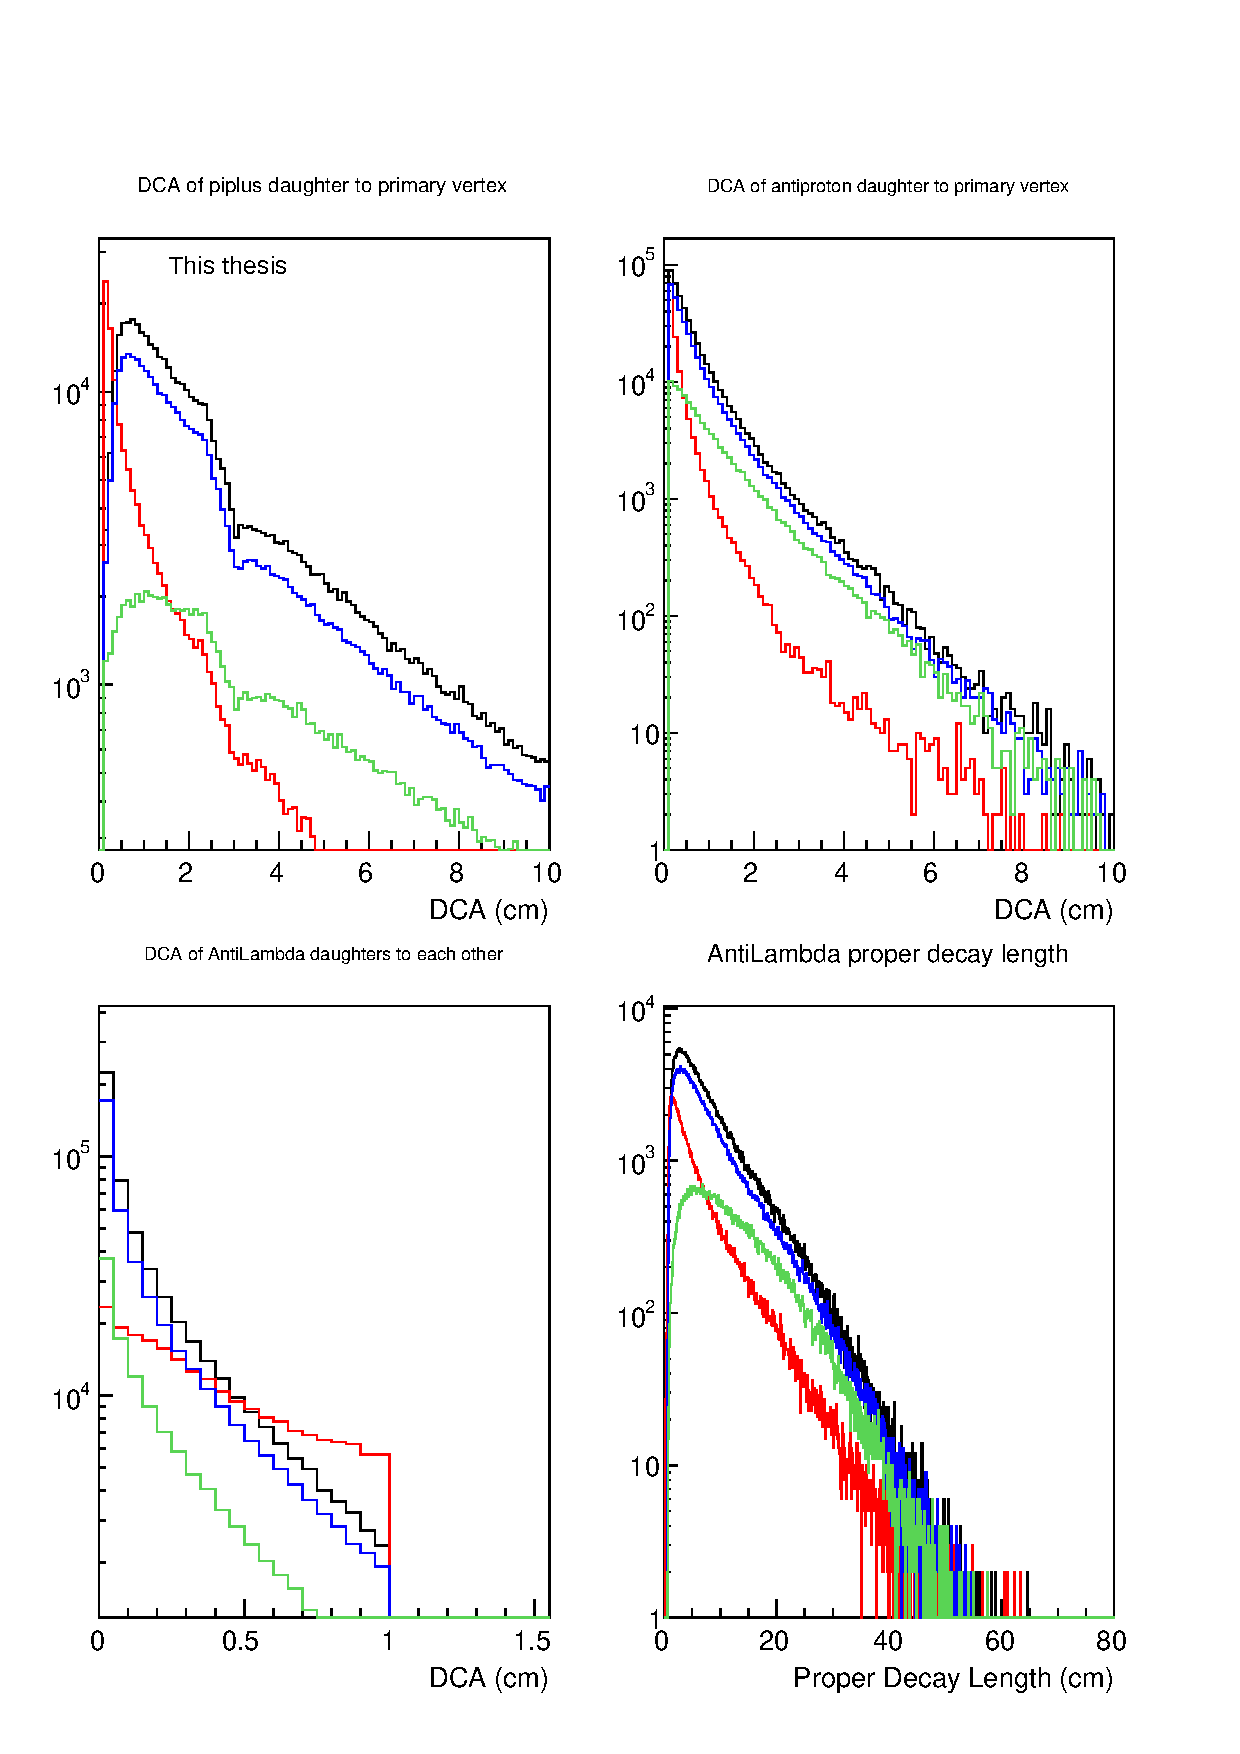
\includegraphics[width=36pc]{Figures/2014-03-31-Distribution-AntiLambda-4Types-DCA-DCA-DCA-DecayLength.pdf}
\caption[$\bar{\Lambda}$ cut distributions]{$\bar{\Lambda}$ cut distributions shown for real $\bar{\Lambda}$ (black), $\bar{\Lambda}$ from $\Sigma$ decay (blue), secondary $\bar{\Lambda}$ from other sources (green), fake $\bar{\Lambda}$ (red). 
Optimal cut values were set such that a looser cut would differentially add more fake and (non-$\bar{\Sigma}$) secondary $\bar{\Lambda}$ than primary $\bar{\Lambda}$}
\label{fig:AntiLambdaCutDists2}
\end{figure}

For the construction of Figures \ref{fig:LambdaCutDists1},\ref{fig:LambdaCutDists2},\ref{fig:AntiLambdaCutDists1}, and \ref{fig:AntiLambdaCutDists2}, each $\Lambda$ type was preselected using AliAODMCParticle information, and only V0 candidates of that type were reconstructed in that analysis run. 
This was done for ease of histogramming the distributions.  
Roughly equal numbers events were analyzed for each run type, with the exception of the analysis of the primary $\Lambda$.  That analysis run utilized only about half the data set.  
Therefore, the primary $\Lambda$ ($\bar{\Lambda}$) distributions in Figures \ref{fig:LambdaCutDists1},\ref{fig:LambdaCutDists2},\ref{fig:AntiLambdaCutDists1}, and \ref{fig:AntiLambdaCutDists2} have been scaled by a factor of 2 to compensate.

In these figures, both the shape and magnitude of each distribution is relevant for determining the cuts. 
For each cut type, a cut value was selected such that a looser cut would differentially accept more fake or secondary $\Lambda$ than primary $\Lambda$. 
Ideally, these cuts would be selected to reduce the inclusion of all types of secondary $\Lambda$.  
However, it can be seen from the distributions that $\Lambda$ that come from $\Sigma$ decay display virtually the same cut parameter distribution shapes as primary $\Lambda$.  
Only the magnitude of the $\Sigma$ curves differ from the primary $\Lambda$ curves.  
This is due to the short decay length of the $\Sigma$ decay: $c\tau \approx 20$ pm for $\Sigma^0$ , and $c\tau \approx 6$ fm for $\Sigma$(1385). 
As a result, secondary $\Lambda$ from $\Sigma$ look identical to primary $\Lambda$ from the perspective of topological cuts, and they cannot be selectively removed from the analysis.

The systematic errors associated with these cut choices are discussed in Section \ref{sec:SystematicsReconstruction}. 
Further discussion of the reconstruction efficiency of the different $\Lambda$ types can be found in Section \ref{sec:ReconstructionEff}.

The reconstructed invariant mass distribution for $\Lambda$ and $\bar{\Lambda}$ can be seen in Figures \ref{fig:LamInvMass} and \ref{fig:ALamInvMass}. 
An approximation of the signal purity was estimated using a ratio of real and background (falsely reconstructed) counts.  
The background was estimated using a fourth order polynomial.  
The number of real $\Lambda$ was then estimated by counting the bin content and subtracting the background. 
The signal quality was found to be $real/(real + background) \approx 0.95$ for both $\Lambda$ and $\bar{\Lambda}$.
The $\bar{\Lambda}/\Lambda$ ratio is estimated to be about 93\%.

\begin{figure}[hbtp]
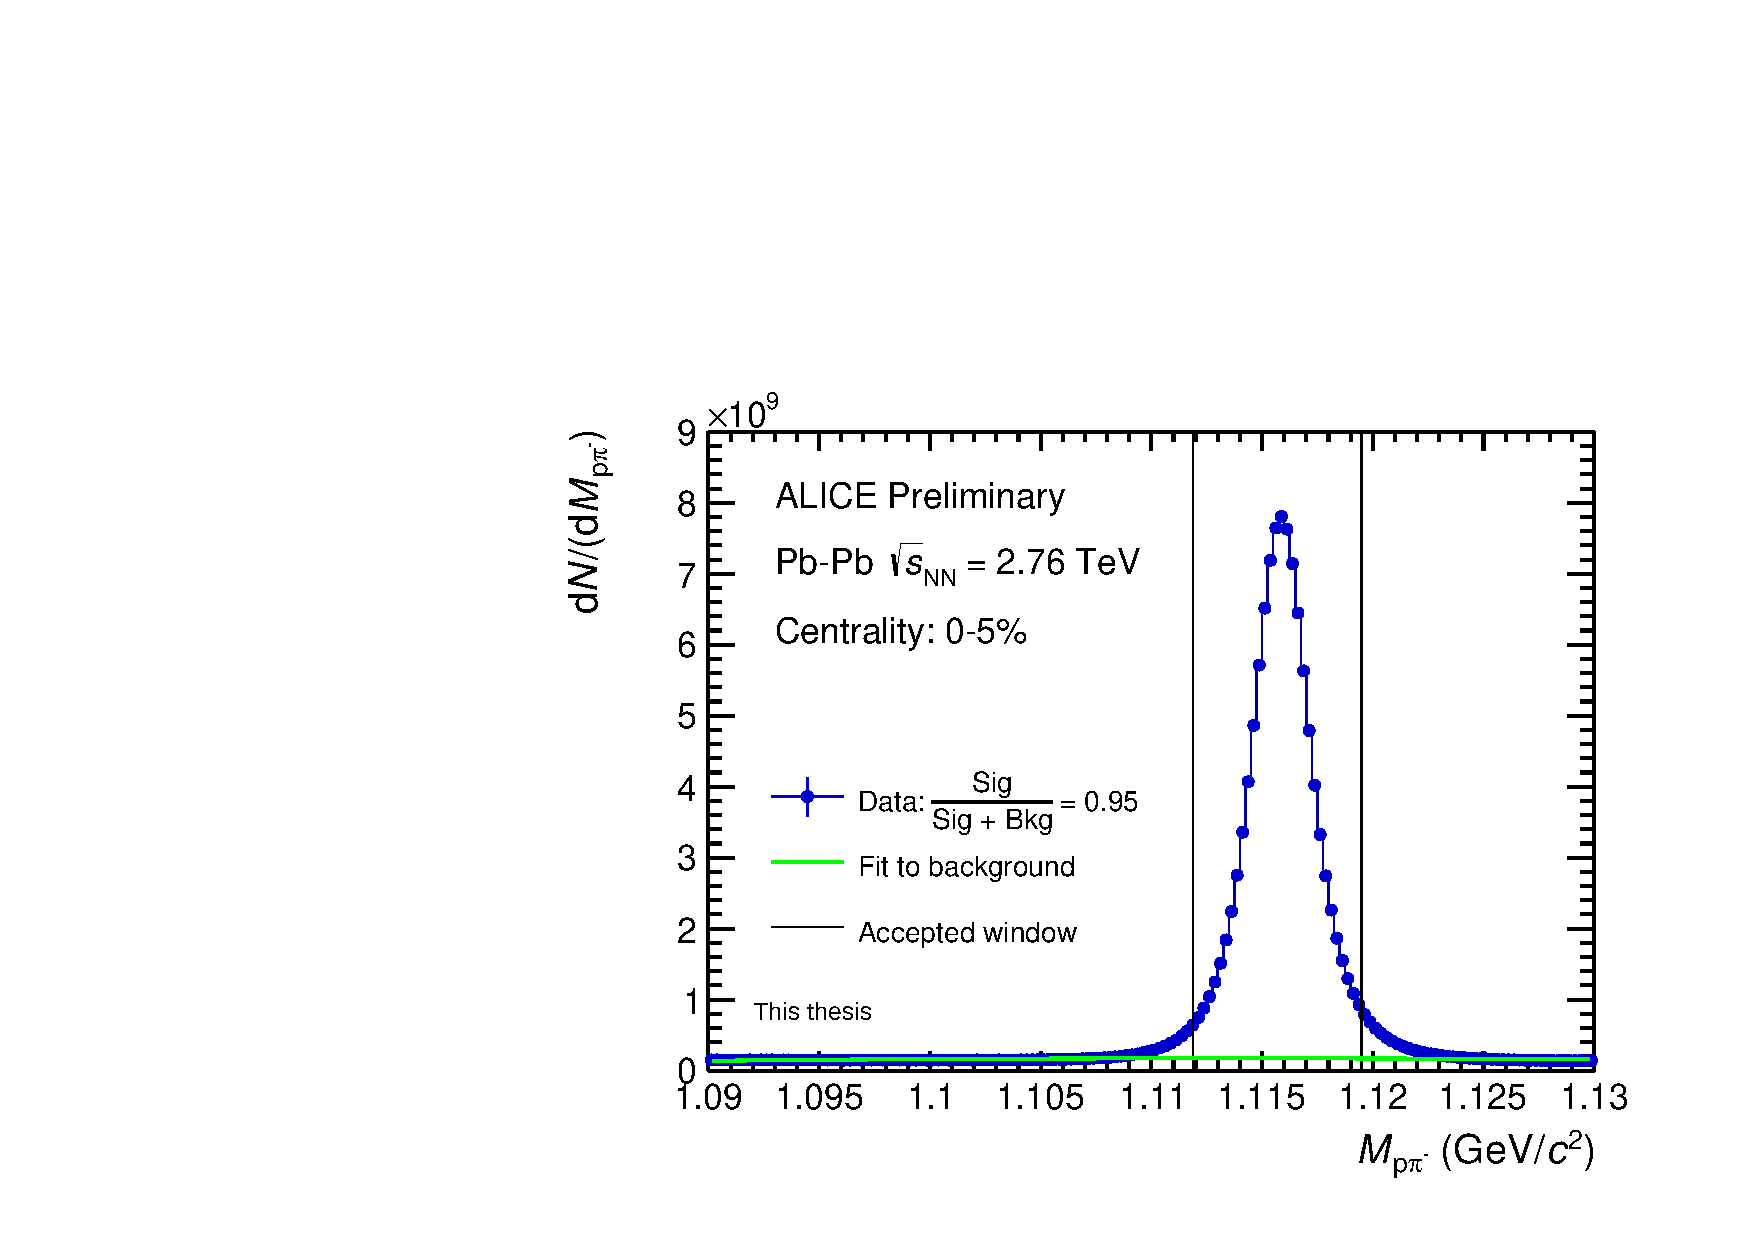
\includegraphics[width=36pc]{Figures/2014-05-11-LamMinv-CommentCorrections.pdf}
\caption[$\Lambda$ invariant mass distribution]{Invariant mass distribution for reconstructed $\Lambda$ using the optimal analysis cuts.  
The plots show V0s reconstructed from centrality integrated LHC11h data.  
The green line shows a fourth order polynomial fit to the background, which is used to estimate the number of real and fake $\Lambda$.  
The estimated ratio of real $\Lambda$ to all reconstructed $\Lambda$ in the signal region ($ \lvert m_{\mathrm{inv}} - m_{\mathrm{PDG}}\rvert < 3.8$ MeV/$\rm c^2$) is approximately 0.95.}
\label{fig:LamInvMass}
\end{figure}

\begin{figure}[hbtp]
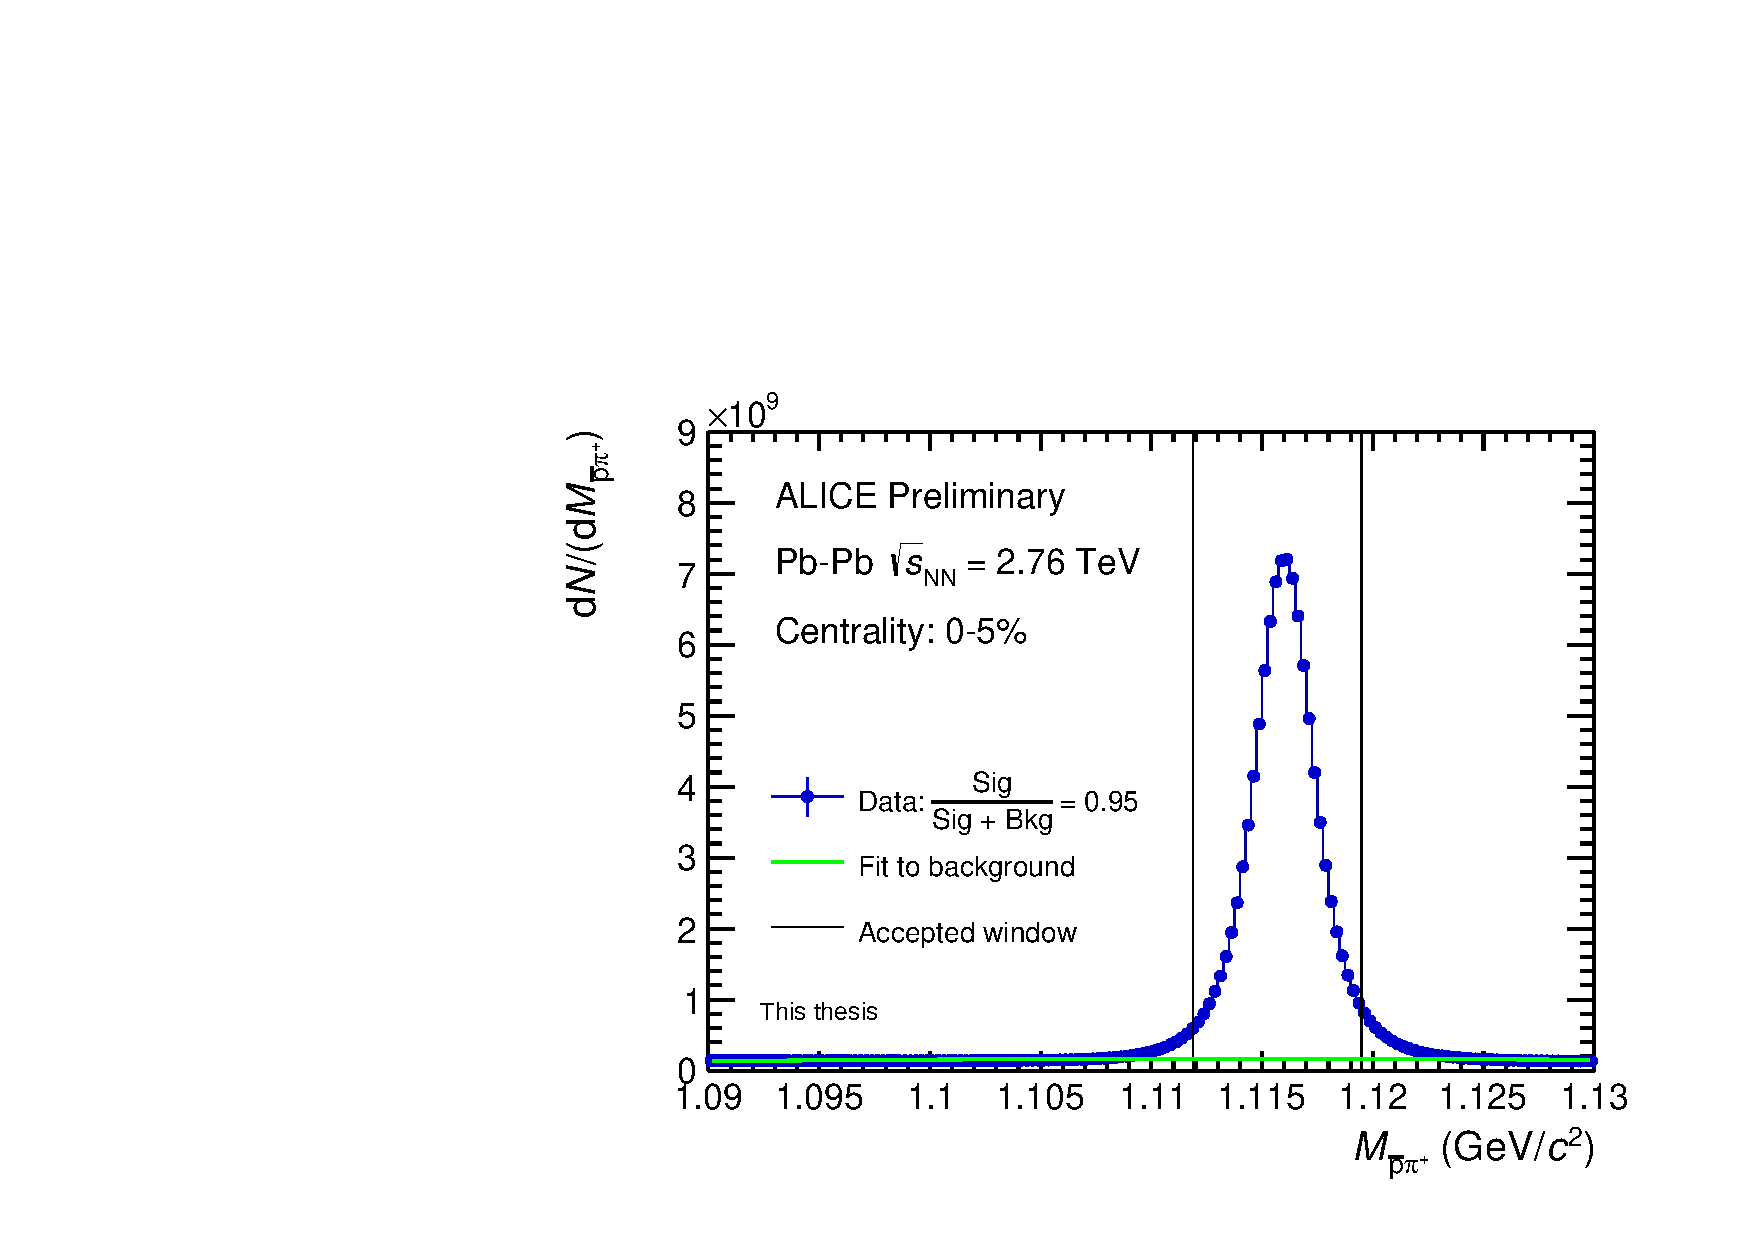
\includegraphics[width=36pc]{Figures/2014-05-11-ALamMinv-CommentCorrections.pdf}
\caption[$\bar{\Lambda}$ invariant mass distributions]{Invariant mass distribution for reconstructed $\bar{\Lambda}$ using the optimal analysis cuts.  
The plots show V0s reconstructed from centrality integrated LHC11h data.  
The green line shows a fourth order polynomial fit to the background, which is used to estimate the number of real and fake $\bar{\Lambda}$.  
The estimated ratio of real $\bar{\Lambda}$ to all reconstructed $\bar{\Lambda}$ in the signal region ($ \lvert m_{\mathrm{inv}} - m_{\mathrm{PDG}}\rvert < 3.8$ MeV/$\rm c^2$) is approximately 0.95.}
\label{fig:ALamInvMass}
\end{figure}

\subsubsection{Decay radius (XY) cut}
The V0 finder includes a default decay radius cut of 0.9 cm, which removes V0s with a radial decay length less than that value.  
This helps mitigate issues such as high track density which can complicate reconstruction.  
This analysis only uses the default cut, though it is possible that a tighter cut could yield improved $\Lambda$ purity without severely impacting the available statistics.  
Changes in this cut are expected to have only small effects on the correlation functions themselves.  
As will be described later in this note, fits of correlation functions have a $\lambda$ parameter which accounts for the pair-purity (roughly the square of the single particle purity).  
In any case, a few percent increase in purity should not drastically impact the shape of the correlation functions.
Studies of this cut may improve V0 selection for future analyses.

\subsubsection{Shared daughter cut}

Occasionally two or more V0s are reconstructed that both claim the same daughter track.  
However, a given track can only be the daughter of, at most, one V0.  
Therefore, if several reconstructed V0s all lay claim to the same daughter, at most only one of them can be a true V0.  
It was decided to employ a cut that would compare characteristics of the different V0s to determine which of them was most likely to be the true parent particle.  
After the best V0 was found, the competing V0s were removed from the list of V0 particles and not used during same- or mixed-event pair construction.

A study was done using MC event truths to determine which cut would be most successful at removing fraudulent V0s.  
The following characteristics were examined as candidates for the cut criterion:

\begin{itemize}
\item Closeness of invariant mass to the PDG mass value.
\item DCA of the daughter particles to each other.
\item Cosine of the pointing angle.
\item DCA of the V0 to the primary vertex.
\end{itemize}

The process of culling V0s with shared-daughters was done by looping through V0s on an event-by-event basis after the V0 reconstruction process was completed.  
For each V0 in the list of successfully reconstructed V0s (i.e. V0s that passed all cuts), the V0 was compared with each other V0 in the event to determine if they shared a daughter.  
Two V0s "share" a daughter if both V0s have a charged daughter track with the same track ID.  
When two V0s were found that shared a daughter, their values of the cut criterion were compared.  
The daughter with the stricter value (e.g.\ smaller DCA to primary vertex) was adjudged to be the better V0 candidate, and the other V0 was flagged as "bad" for failing the shared-daughter cut.  
V0s that failed the shared-daughter cut were not used in any pair construction (same event or mixed event).

However, it is possible for a V0 to share a daughter or daughters with two different V0s. 
In the aforementioned scheme, it is therefore possible for an excessive number of V0s to fail the shared daughter cut (excessive in that some of those failed V0s only shared a daughter with another failed V0).  
To avoid throwing away too many V0s, a second loop was added to shared-daughter cut method to un-flag V0s that no longer share a daughter with any "good" V0. 
Example: V0s "A" and "B" both share a daughter, and V0s "A" and "C" share a different daughter.  "A" has a better DCA than "B", so "B" is flagged as bad.  
Then "C" is found to have a better DCA than "A", so "A" is flagged as bad.  
Finally, "B" is re-flagged as good because it no longer shares a daughter with any other good V0.

This method was adapted to run iteratively over the list of V0s candidates until a stable list of non-sharing V0s was found.  
Then the MC truths of each V0 (those marked "good" and those marked "bad") were examined.  
With this information, it is possible to calculate the percentages of true V0s and fake V0s that are removed via this process.  
This analysis was run several times, each time using a different comparison criterion from the list above.

Based on the MC truth study, keeping the V0 with the closest DCA to the primary vertex was found to successfully keep 87\% of true V0s that had shared daughters.  
In comparison, the cosine of pointing angle criteria was also successful 87\% of the time (cos$(\Theta_\mathrm{p})$ and DCA to primary vertex are strongly correlated), the DCA of daughters to each other criteria was successful 81\% of the time, and the absolute value of mass difference criteria was successful 79\% of the time.
Based on these results, the DCA to primary vertex criteria was selected to used for the shared-daughter cut before correlation function construction.

%On average there were two competing particles per every ... events in the MC study.  When applied to analysis of the LHC11h data, the rate was two per ....

One of the benefits of this cut is that it helps remove a splitting-like effect (see Section \ref{sec:PairWiseCuts} for more on splitting), wherein a true V0 shares each of its daughters with two separate fake V0s.  
By the nature of the reconstruction cuts, all three of the V0s will be close in momentum space.  
Therefore a pair constructed from the two fake V0s will contaminate the low relative-momentum region of the correlation function.  
That pair of fake V0s does not share any daughters with each other, so it is not kept out of the correlation function by simple daughter ID checks.  
But the iterative daughter-sharing cut described above is capable removing this fraudulent pair, since either of the fake V0s is likely to be removed for sharing a daughter with the true V0.

\section{Correlation function construction}
\label{sec:CorrelationFunctionConstruction}
\subsection{Relative momentum}
\label{sec:RelativeMomentum}

This analysis studies two-particle correlations as a function of the one-dimensional relative momentum $k^*$.
To be precise, for a pair of particles with four-momenta $p_1$ and $p_2$, $k^*$ is the momentum of one the particles in the pair's center of mass frame.
It is defined as
\begin{equation}
\label{eq:kstar}
k^*= \sqrt{-k^\mu k_\mu},
\end{equation}
where $k^\mu$ is half of the four-vector relative momentum
\begin{equation}
\label{eq:kmu}
k^\mu = \frac{p_1^\mu - p_2^\mu}{2} -\frac{(p_1 - p_2)\cdot P}{2P^2}P^\mu,
\end{equation}
$P$ is the four-vector momentum sum.

The literature is inconsistent when it comes to the notation for relative momentum.
In some cases, $k^*$ refers both to the invariant quantity and to the four-vector.
In this thesis, we will try to consistently use $k^*$ to designate the invariant quantity, and use $k^\mu$ when speaking of four-momenta.
In some papers, $q$ or $q_{\mathrm{inv}}$ is used to represent the relative momentum.
Though we won't use $q$ in this analysis, for reference
$q^\mu = 2k^\mu$, and $q_{\mathrm{inv}} = 2 k^*$.


\subsection{Construction}
\label{sec:CFconstruct}

The correlation function is constructed as
\begin{equation}
\label{eq:CFDefinition}
C(k^*) = \frac{A(k^*)}{B(k^*)},
\end{equation}
where $A(k^*)$ is the two-particle distribution of the given event and $B(k^*)$ is the distribution of a reference event.  
In practice, the signal event histogram $A(k^*)$ is constructed by binning the $k^*$ value of each pair of particles in a single event, and repeating this for each event.  
The reference or background histogram is constructed by binning $k^*$ for pairs of particles taken from different events.  
The correlation function therefore is the ratio of the two-particle phase-space with correlated effects coming from interactions (the numerator) to the two-particle phase-space without correlated effects (the denominator).
Because the denominator pairs are uncorrelated, their two-particle phase space is essentially a convolution of two single-particle phase spaces.
Of course, the numerator pairs are also affected by the single-particle phase spaces.
We assume that the physics of the numerator pairs can be factorized to separate out the correlated physics effects and the single-particle phase space effects.
Thus, dividing by the background pair distribution leaves us with just the correlated physics effects, i.e.\ the correlation function. See Section \ref{sec:KooninPratt} for more details.

In order for the phase-space effects to divide out, it is of course necessary for the mixed events to resemble the true events.
For example, a mixed event where half the particles come from a central collision and half the particles come from a very peripheral collision would have a very different two-particle phase space than a central collision would.
Care is therefore taken to ensure that pairs are mixed from events with similar characteristics. 
Mixed events are required to have approximately the same centrality (bin width of 5\%) and primary vertex z-position (2 cm bin width).  
There are approximately five mixed events for each real event.  
When constructing pairs of V0s from the same event, the V0s are not allowed to share a daughter with the same track ID. 
The correlation functions are normalized to unity in the $ 0.3 < k^* < 0.5$ GeV/c range.

\subsection{Pair cuts}
\label{sec:PairWiseCuts}

Femtoscopic studies look at the relative momentum of particles, and often the most interesting physics lies at very low relative momentum (around 0.1 GeV/c and lower).  
As a result, two-track reconstruction effects such as track splitting and track merging, both of which occur for tracks with similar momenta and trajectories, can have a large effect on the measured results.  
Track splitting means that the track left by a single charged particle is reconstructed as two separate tracks. 
A track splitting-like effect can also occur from cutting out tracks with too many shared TPC clusters.
Track merging occurs when the tracks of two separate particles are reconstructed as a single track.  
For V0s, splitting/merging occurs on the level of the daughter tracks, and it affects the reconstruction of the parent V0s.
However, one must be somewhat cautious here, since there can be physics effects that lead to a suppression or enhancement of tracks that are close together.
In particular, small track separation correlates somewhat with small relative momentum, so effects that suppress (enhance) low-$k^*$ pairs may also lead to some suppression (enhancement) of low-average separation pairs.  

In this analysis, two-track reconstruction effects are combated via a cut on the average separation of daughter tracks from different $\Lambda/\bar{\Lambda}$.  
The average separation distance of two daughter tracks are computed at nine different radii of the TPC.  
The track positions are measured via AliExternalTrackParam::GetXYZatR() at the following radii: 85, 105, 125, 145, 165, 185, 205, 225, and 245 cm.  
Pairs of daugther tracks are made from one daughter from the first V0 and one daughter from the second V0. Pairs are made for all daughter combinations, and each type of pair is tracked separately.
For each pair of daughter tracks, their separation is computed at each of those radii, and their average separation is taken as the mean value. If a track does not have a value at a particular radius (e.g.\ a low $p_T$ track with a small radius of curvature), that position is excluded from the calculation of the mean.
Same- and mixed-event pairs are binned according to this separation distance.  
To obtain an estimate of the merging/splitting effects both distributions are then scaled by the number of pairs at high average separation distance (10+ cm), and a correlation function (same event pairs/ mixed event pairs) is created. 

To ensure that average separation distributions of mixed-event pairs are comparable to the same-event distributions, it is necessary to perform a shifting of the primary vertex for mixed events.  
Doing so allows the track separations to be calculated as though both events had the same primary vertex.  
Without this correction, the mixed-event distributions are biased by differences in the primary vertex location.  
One could imagine an extreme example of this if one used a 20 cm wide z-vertex bin.  
In that case, tracks from different events could be shifted relative to each other by as much as 20 cm. 

The average separation correlation functions for various V0 daughter combinations are available in Figure \ref{fig:AverageSeparationAllPairs}.  
We see that all like-sign pair combinations, as well as proton-antiproton, show a dip at low average separation.  
This dip tells us that there is a depletion of tracks that are close together. 
This depletion may come from track merging or from effects similar to track merging, such as the rejection of tracks that have too many shared TPC clusters.
For these pairs of tracks, we implement cuts at average separation value where the correlation function looks to reach unity.
These cuts are applied uniformly to same-event and mixed-event pairs.
pp and $\bar{\mathrm{p}}\bar{\mathrm{p}}$ pairs are cut if their separation lies below 12 cm, while $\pi^-\pi^-$, $\pi+\pi^+$, p$\pi^+$, $\bar{\mathrm{p}}\pi^-$ and p$\bar{\mathrm{p}}$ are cut below 10 cm.

For the other opposite-sign pairs, the splitting/merging picture is less clear, in great part due to the low statistics at low average separation.
First and foremost, this tells us that there is a very low phase space for finding oppositely charged particles. 
That should not be a surprise, as the ambient magnetic field accelerates them in opposite directions.
As it is not clear whether there exists splitting or merging from these pairs, a conservatively large average separation cut has been implemented. p$\pi^-$ and $\bar{\mathrm{p}}\pi^+$ are cut at 15 cm, and $\pi^-\pi^+$ are cut at 25 cm.

One alternative/complement to using an average separation cut would be to enforce a relative decay length cut, where V0s are not paired with each other if their difference between their lab frame decay length values is less than some cut value (e.g.\ a few cm).  
One advantage of this cut is that the decay lengths of the various particles should be independent of physics effects - i.e. independent of any quantum interference or final state interaction that might occur between the particles.  
Meanwhile, the decay length cut may minimize daughter splitting effects, as well as some merging of low- and mid-$p_{\mathrm{T}}$ daughters.  
High-$p_{\mathrm{T}}$ daughters may still be affected by merging, since higher-$p_{\mathrm{T}}$ particles have straighter trajectories in the TPC.  
A study of relative decay length has not been performed here, but it may prove useful to combat splitting/merging effects in future V0 analyses.

\begin{figure}[hbtp]
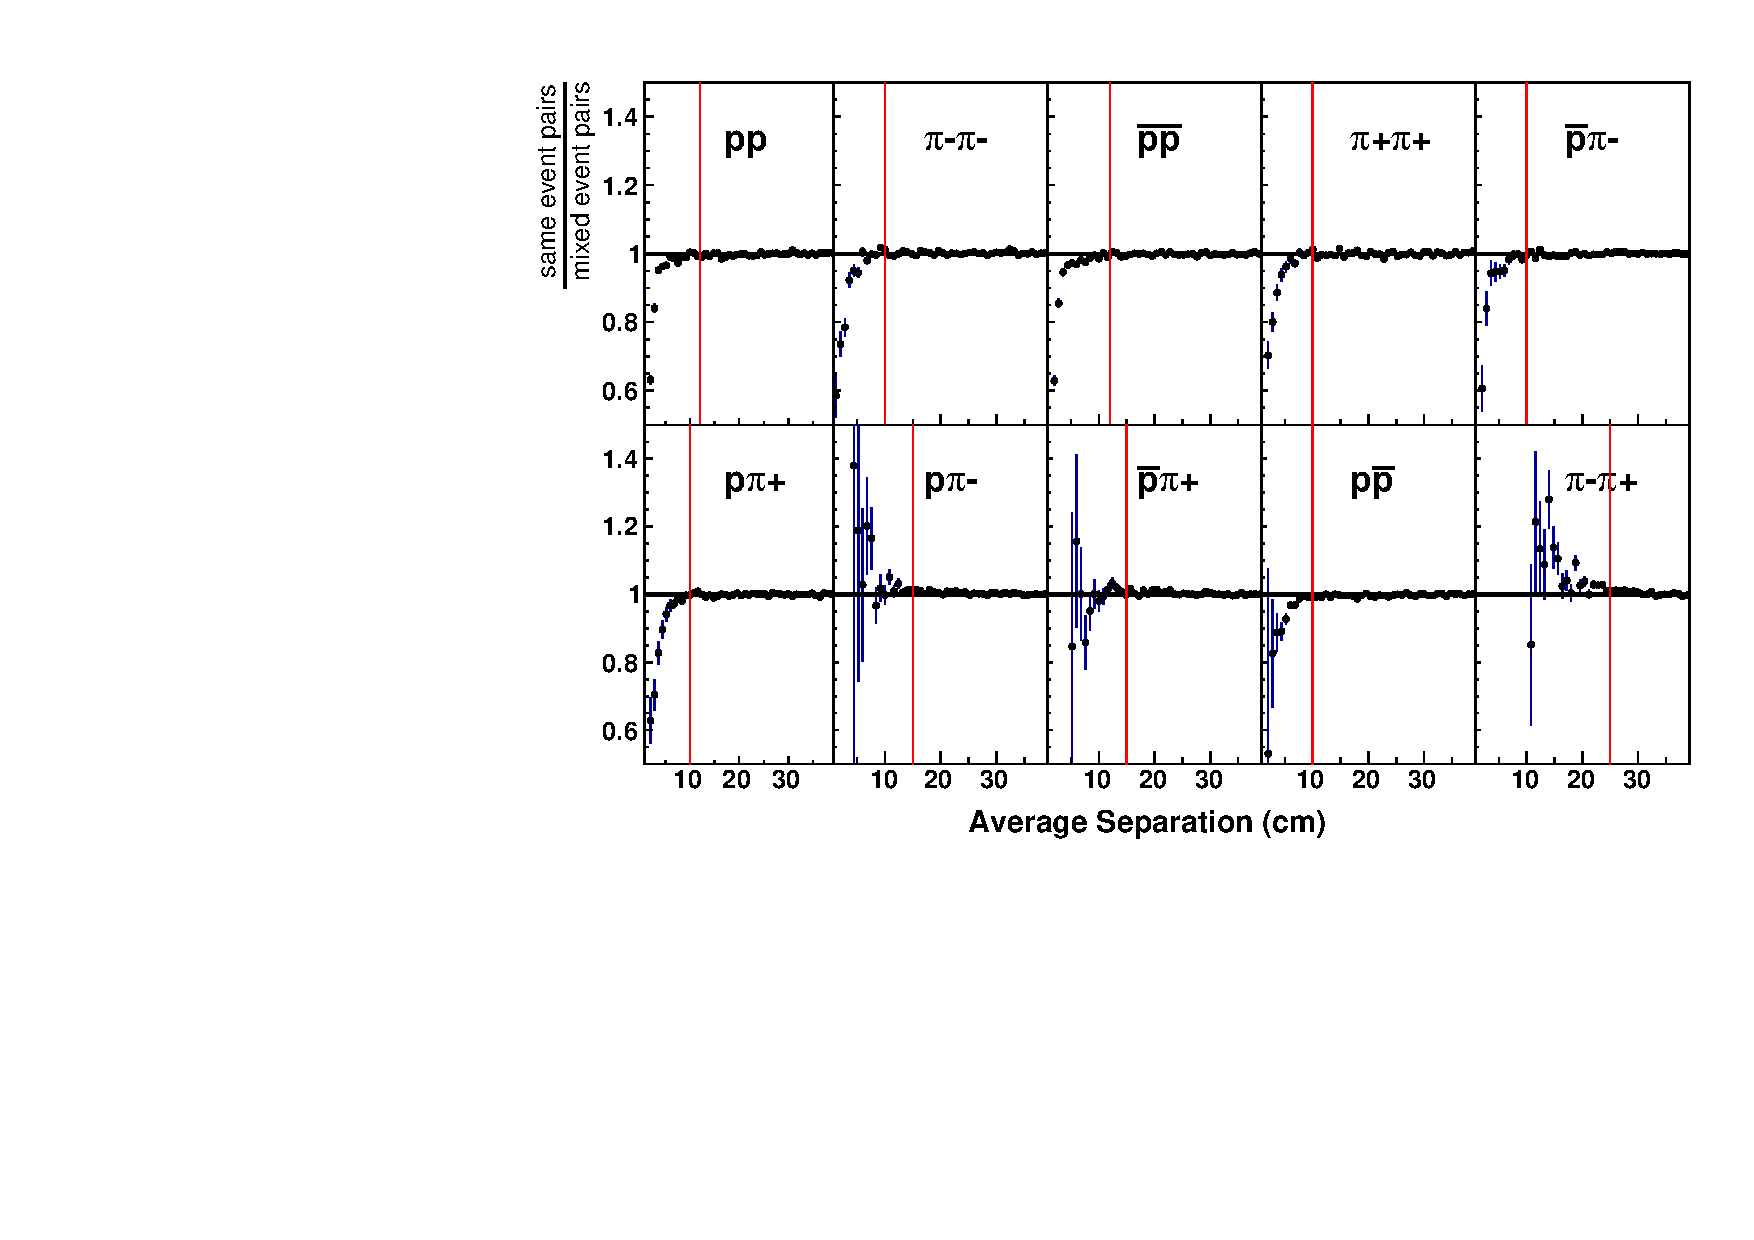
\includegraphics[width=36pc]{Figures/Cuts/2016-9-4-AllAvgSepCFs.pdf}
\caption[Average separation of V0 daughters]{
Correlation functions of average TPC track separation for pairs of daughters from different V0s. A correlation function is shown for each type of daughter combination. The positions of tracks are computed throughout the TPC, and an average separation value is calculated from those positions. This process is done for same- and mixed-event pairs. The correlation function reveals merging-like effects for all same-sign pairs and also for p$\bar{\mathrm{p}}$. To remove splitting/merging effects, V0 pairs are cut if  their daughters' average separation is below the indicated red line. Conservatively large cuts have been implemented for oppositely-charged pairs.}
\label{fig:AverageSeparationAllPairs}
\end{figure}

\subsection{Momentum resolution correction}
\label{sec:MomentumResCorrectionCF}

There is an inherent resolution to V0 momenta that depends on the resolution of the reconstructed daughter tracks.  
Because of this limit of precision, there is also an associated resolution to the relative momentum of two V0s.
This causes the reconstructed relative momentum of the pair to differ from the true momentum of the pair, and it therefore introduces subtle changes to the measured correlation functions which must be accounted for.

Tradionally, the momentum resolution correction is performed on the experimental data to unsmear it into a form that should resemble the theoretical predictions (i.e.\ fits). 
In this analysis we have instead chosen to smear the fits to conform to the experimental data. 
The experimental correlation functions therefore remain uncorrected. 
As our corrections are employed at the time of fitting, we'll discuss the full methodology in section \ref{sec:MomResCorrectFit}.
\section{Systematic uncertainties of correlation functions}
\label{sec:SysUncertaintyCF}

We will now attempt to identify the various systematic effects that may affect the correlation functions.  
The goal will be to quantify the systematic uncertainties associated with each $k^*$ bin.  
It should be noted, however, that subsequent fits to the correlation functions are not directly impacted by these error bars.  
Instead, the systematics on the resulting fit parameters will be computed by refitting many versions of the correlation functions (e.g.\ those built with different reconstruction cuts) and comparing the results. 
This will be discussed in greater detail in Section \ref{sec:SysErrorsFitsCuts}.

\subsection{Consistency checks for uncorrelated histograms}
\label{sec:ConsistencyCheckUncorrelated}
One of the tools we employ in the search for systematic effects is the TH1::Chi2Test(TH1* h1) method, which compares two histograms bin-by-bin to determine a $\chi^2$.  
The test is performed assuming the hypothesis that the two histograms are Poissonian samples of the same underlying distribution.  
A p-value is computed which represents the probability that a measurement could be performed that would yield results this different or more, given the hypothesis of identity.  
The hypothesis of identity is rejected in instances where the p-value is lower than 0.01. 
At that threshold, less than one percent of tests will fail of data sets sampled from the same underlying distribution.  
This corresponds to rejecting the hypothesis of identity for data samples that differ by roughly $3 \sigma$.  
The 0.01 metric is somewhat arbitrary - it was chosen to be small enough that pure statistical fluctuations should not often lead to false or unnecessary systematic errors.  
For example, if a p-value of 0.1 were used instead, this would result in roughly 10\% of "good" results failing the test and contributing to the uncertainty, which would lead to a gross overestimation of the total systematic error.  
Similarly, a threshold of 0.001 would probably underestimate the error.  
Thus, 0.01 was chosen.

In this analysis, Chi2Test() will be used to compare two correlation functions which are uncorrelated with each other (uncorrelated in the sense that they are completed independent data samples).  
One example where this can be employed is the comparison of correlation functions constructed using data taken under different field configurations.  
This analysis needs all the data available to it, so results taken under different field configurations will need to be merged to improve statistics.  
But before they are combined, it must be checked that they contain compatible results.  
The Chi2Test() method provides a means of characterizing the degree of similarity of the correlation functions.  

Correlation functions that surpass the significance level of 0.01 will be treated as being functionally the same within statistics, and their weighted average will be computed without recourse to systematic uncertainty. 
In the instances where they do not exceed the significance level, they will be analyzed on a case-by-case basis.  
In particular, we will look to see if there are any systematic differences between the correlation functions.  
For example, it may be seen that the lowest ten $k^*$ bins will all be higher in one correlation function than another.  
If so, the data will still be merged (so long as the results aren't dramatically different), but a systematic uncertainty will be computed and applied to the final averaged correlation function in the form of systematic error bars.  
%Section \ref{sec:CalculatingSysErrors} describes how these uncertainties are calculated.  

When using Chi2Test() to compare correlation functions, the trouble areas that result in small p-values will likely be the lowest $k^*$ bins (which exhibit most of the interesting physics, and which also suffer the most from two-track effects), and large $k^*$ bins (close to $1 \mathrm{GeV/c}$).  
The height of the the large $k^*$ bins is noticeably susceptible to statistical (or systematic) deviations in the normalization region.  
The high $k^*$ bins have relatively small statistical error bars, so small deviations of normalization between correlation functions can result in large $\chi^2$ values.  
The correlation functions are all normalized to unity in the $0.3 < k^* < 0.5 \mathrm{GeV}/c$ range, so there are unlikely to be significant deviations seen in that range.  

It is important to emphasize that Chi2Test() is only appropriate for comparing two uncorrelated histograms.  
In the case of correlated histograms (e.g.\ correlation functions constructed using slightly different two-track cuts or different reconstruction cuts), a different method must be used to test the histograms for consistency. 

In this analysis, $\chi^2$ tests of correlation functions with different magnetic field configurations found that the results from the two fields were consistent with each other.
Therefore, the magnetic field configurations to not to contribute to the systematic uncertainties on the correlation functions or fit results. 


\subsection{Consistency checks for correlated histograms}
\label{sec:ConsistencyCheckCorrelated}
Chi2Test() cannot be used to compare correlated data because the test is performed assuming the statistical error bars on the two histograms are independent.  
That is obviously not the case for two histograms that differ in their content by only a few percent.  
In this analysis, we follow the advice of Roger Barlow \cite{Barlow:2002yb} and perform consistency checks of correlated data in the following fashion:

\begin{enumerate}
\item Take the difference between the two correlation function histograms $$\Delta C(k^*) = C_1(k^*) - C_2(k^*),$$ using $C_1\rightarrow$ Add($C_2$,$-1$).  
The resulting histogram shows the usually small differences between the two data sets.
\item Here, ROOT adds the errors in quadrature, which isn't correct for correlated data.  
To fix this, we manually set the error bars using $\sigma_{\Delta}(k^*) = \sqrt{ \abs{ \sigma_1^2(k^*) - \sigma_2^2(k^*) }}$.  
This error is correct in the specific case (found here) that one histogram is entirely a subset of the other.
\item We now look to see if there are any significant discrepancies or systematic differences between the two original correlation functions.
If there is a structural difference, it will generally be largest in the lowest $k^*$ bins, dropping off as $k^*$ increases.
This shape is reasonably described by a decaying exponential: $f(k^*) = a \exp(-b k^*)$. 
The amplitude $a$ tells us the size of the discrepancy. The width $b$ has no significance; it just helps the fit.
\item We fit the histogram with the exponential, and we extract the amplitude $a$ and its error $\sigma_a$.
For this analysis, we conclude that there is no discrepancy if $a$ is within 2$\sigma$ of zero.
If $a$ is more than 2$\sigma$ from zero, then we have a source of systematic uncertainty.
\item In the cases where there is a systematic deviation, we take the height of the fit function in the center of each $k^*$ bin as the systematic uncertainty for that bin from this cut.
As the fit function can be positive or negative, this leads to asymmetric errors.

\end{enumerate}

Using the steps listed above, we can evaluate if seemingly small changes to the cuts employed in correlation function construction change the resulting data in any significant way.  


\subsection{Systematic errors from reconstruction cuts}
\label{sec:SystematicsReconstruction}

In this section we discuss the systematic errors associated with the V0 reconstruction cuts (e.g.\ cosine of pointing angle, DCA to primary vertex, etc.).  
Loosely speaking, these systematic checks test the sensativity of the correlation function to small changes in the $\Lambda$ purity.
The optimal cut values were discussed in Section \ref{sec:Recon}.  
For example, the optimal cut value chosen for the DCA of daughter tracks to each other was 4 mm (daughters tracks were required to pass within that distance of each other).    
However, there is some ambiguity in determining the optimal cut value.  
For example, any value within $4\pm10\%$ would be reasonable.
The correlation function should ideally be insensitive to small changes in the cut value.
If a small tweak to the cut values produces a statistically significant change in the correlation function, that is a source of systematic uncertainty.

To test for systematic differences, we make correlation functions using $\Lambda$ ($\bar{\Lambda}$) reconstructed with these different cut values. 
At any given time, one cut type (e.g.\ DCA of proton daughter to primary vertex) will be varied away from the default cut value by $\pm10\%$, while the other cut types (e.g.\ cosine of pointing angle) are fixed to their default values. 
  
Data has been collected for variations of the following cuts: 
\begin{itemize}
\item DCA of proton daughter to primary vertex
\item DCA of pion daughter to primary vertex
\item DCA of daughters to each other
\item Proper decay length of $\Lambda$
\item Eta of $\Lambda$
\item Cosine of $\Lambda$ pointing angle
\item DCA of the $\Lambda$ to primary vertex
\item $p_{\mathrm{T}}$ of $\Lambda$
\item Reconstructed mass ($m_{\pi\mathrm{p}}$)
\end{itemize}
  
In each case, correlation functions have been constructed for each pair type ($\Lambda\Lambda$, $\bar{\Lambda}\bar{\Lambda}$, and $\Lambda\bar{\Lambda}$), and for the three cut values (optimal cut, cut + 10\%, cut - 10\%).  
The optimal cut correlation functions are compared with the tighter and looser cut correlation functions.  
The correlation functions all share much of the same data, so they are highly correlated with each other.  
We therefore analyze the changes in the correlation function using the method described in Section \ref{sec:ConsistencyCheckCorrelated}.

Checking each cut yields a positive, negative, or non-existent systematic uncertainty from that cut for each $k^*$ bin. 
For a given bin, we take the positive and negative values with the largest magnitude to be the upper and lower asymmetric errors, respectively.


\subsection{Systematic errors from pair-wise cuts}
\label{sec:SystematicsPairWise}

The systematic uncertainties from the average separation cut are implemented in exactly the same way as the single-particle reconstruction cuts in the previous section. 
For each cut value, we vary the cut by $\pm10\%$, construct correlation functions, and find the uncertainty for each $k^*$ bin via the method in Section \ref{sec:ConsistencyCheckCorrelated}.
In general, the systematic uncertainties are quite small --- about an order of magnitude smaller than the uncertainties from the reconstruction cuts.

\subsection{Systematic errors from shared-daughter cut}

At this time, two femtoscopic analyses at ALICE employ a shared-daughter cut (this analysis and the $\mathrm{K}^0_\mathrm{S}$ analysis), though each cut is implemented with independent code.  
The reasons for this cut are intuitive - two V0s cannot actually have the same daughter, regardless of what might arise from the reconstruction process.  
Moreover, the efficacy of the cut is high: the MC studies of this cut have shown that only 13\% real V0s with shared daughters are cut.  
The removal of a V0 (real or fake) removes all of the same-event and mixed-event pairs that would have included that V0.  
In most cases, this amounts to an improved purity of the correlation function, since there are fewer pairs of fake and therefore uncorrelated particles.  
There also a removal of a splitting-like effect - in this case the "split" is an extra V0 close in momentum space to the first.  
While the two "split" V0s will never be paired together, both are paired with other V0s, resulting in extra pair counts in roughly the same $k^*$ bins.  
Those extra pairs are removed by virtue of the shared daughter cut.

While the benefits of the shared-daughter cut are apparent,
and the disadvantages seem to be minimal (even when you cut a real V0, you a left with a fake V0 that is close in phase space), it is unclear at this time how to determine what systematic uncertainties may arise from this cut and how to quantify that uncertainty.

\subsection{Combining different sources of systematic error}
\label{sec:CombiningSys}

Systematic errors have been evaluated for reconstruction cuts and average separation cuts.
The reconstruction cuts and the separation cuts both yield asymmetric errors for each $k^*$ bin of the correlation function.
We then add those asymmetric errors in quadrature (positive with positive, negative with negative) to get the full systematic uncertainty on the correlation functions.
The resulting correlation functions with combined systematic errors are shown in Section \ref{sec:CorrelationFunctionResults}.
For all correlation functions and all $k^*$ bins, the systematic uncertainties are much smaller than the statistical error bars.


\section{Correlation function results}
\label{sec:CorrelationFunctionResults}
\subsection{Combining correlation functions}
\label{sec:CFCombining}

Correlation functions have been constructed using the entirety of the LHC11h data set.  
As discussed in Section \ref{sec:CFconstruct}, events were binned in 5\% centrality bins.  
When combining data from different centrality bins, care was taken to combine the correlations by taking weighted averages of the correlation functions.  

The naive method of combining correlation functions involves adding numerators from different bins and adding denominators from different bins and then taking the ratio.  
However, this has the pitfall of potentially combining drastically different phase spaces.  
As a result, it may introduce artificial signals into the combined correlation function.  
Instead of using this method, a more correct method is to construct correlation functions for different bins separately.  
Then one takes a weighted average of the correlation functions, using the number of numerator pairs in each correlation function as the weight:

\begin{equation}
\label{eq:CombineCF}
C_{combined}(k^*) = (\displaystyle\sum\limits_{i} w_i C_i(k^*))/(\displaystyle\sum\limits_{i} w_i)
\end{equation}
where the sum is done over different correlation function bins (e.g.\ 0-5\% and 5-10\%) and $w_i$ is the number of numerator pairs in $C_i$.  
This averaging is done on a bin-by-bin basis in $k^*$.  
Note that this averaging procedure should be used in general to combine data sets with potentially different phase spaces. 
For example, this procedure is employed to combine data from runs utilizing the two different field orientations (see Section \ref{sec:DataSelection}).  
It is also employed when combining $\Lambda\Lambda$ data with $\bar{\Lambda}\bar{\Lambda}$ data.  
The statistics are too limited to analyze these correlation functions separately. Instead, we combine them together using the above method for better fitting.

For each centrality range (0-10\%, 10-30\%, and 30-50\%), the correlation functions of the two pair types were found to be consistent with each other (p-values of 0.26, 0.02, and 0.43 respectively).  
Therefore, no additional systematic error was assessed to come out of their merging.

Figures \ref{fig:CFLamLamALamALam010}, \ref{fig:CFLamLamALamALam1030STAR}, and \ref{fig:CFLamLamALamALam3050} show combined $\Lambda\Lambda + \bar{\Lambda}\bar{\Lambda}$ correlation functions for the $0-10$\%, $10-30$\%, and $30-50$\% centrality ranges respectively.  
Figures \ref{fig:CFLamALam010}, \ref{fig:CFLamALam1030}, and \ref{fig:CFLamALam3050} show $\Lambda\bar{\Lambda}$ correlation functions for the $0-10$\%, $10-30$\%, and $30-50$\% centrality ranges respectively.  
Each plot includes the combined systematic errors discussed in Section \ref{sec:SysUncertaintyCF}.
All six correlation functions are included in Figure \ref{fig:CFAllOnOnePlot}.
%, which is considered as a possible figure for publication.

\begin{figure}[hbt]
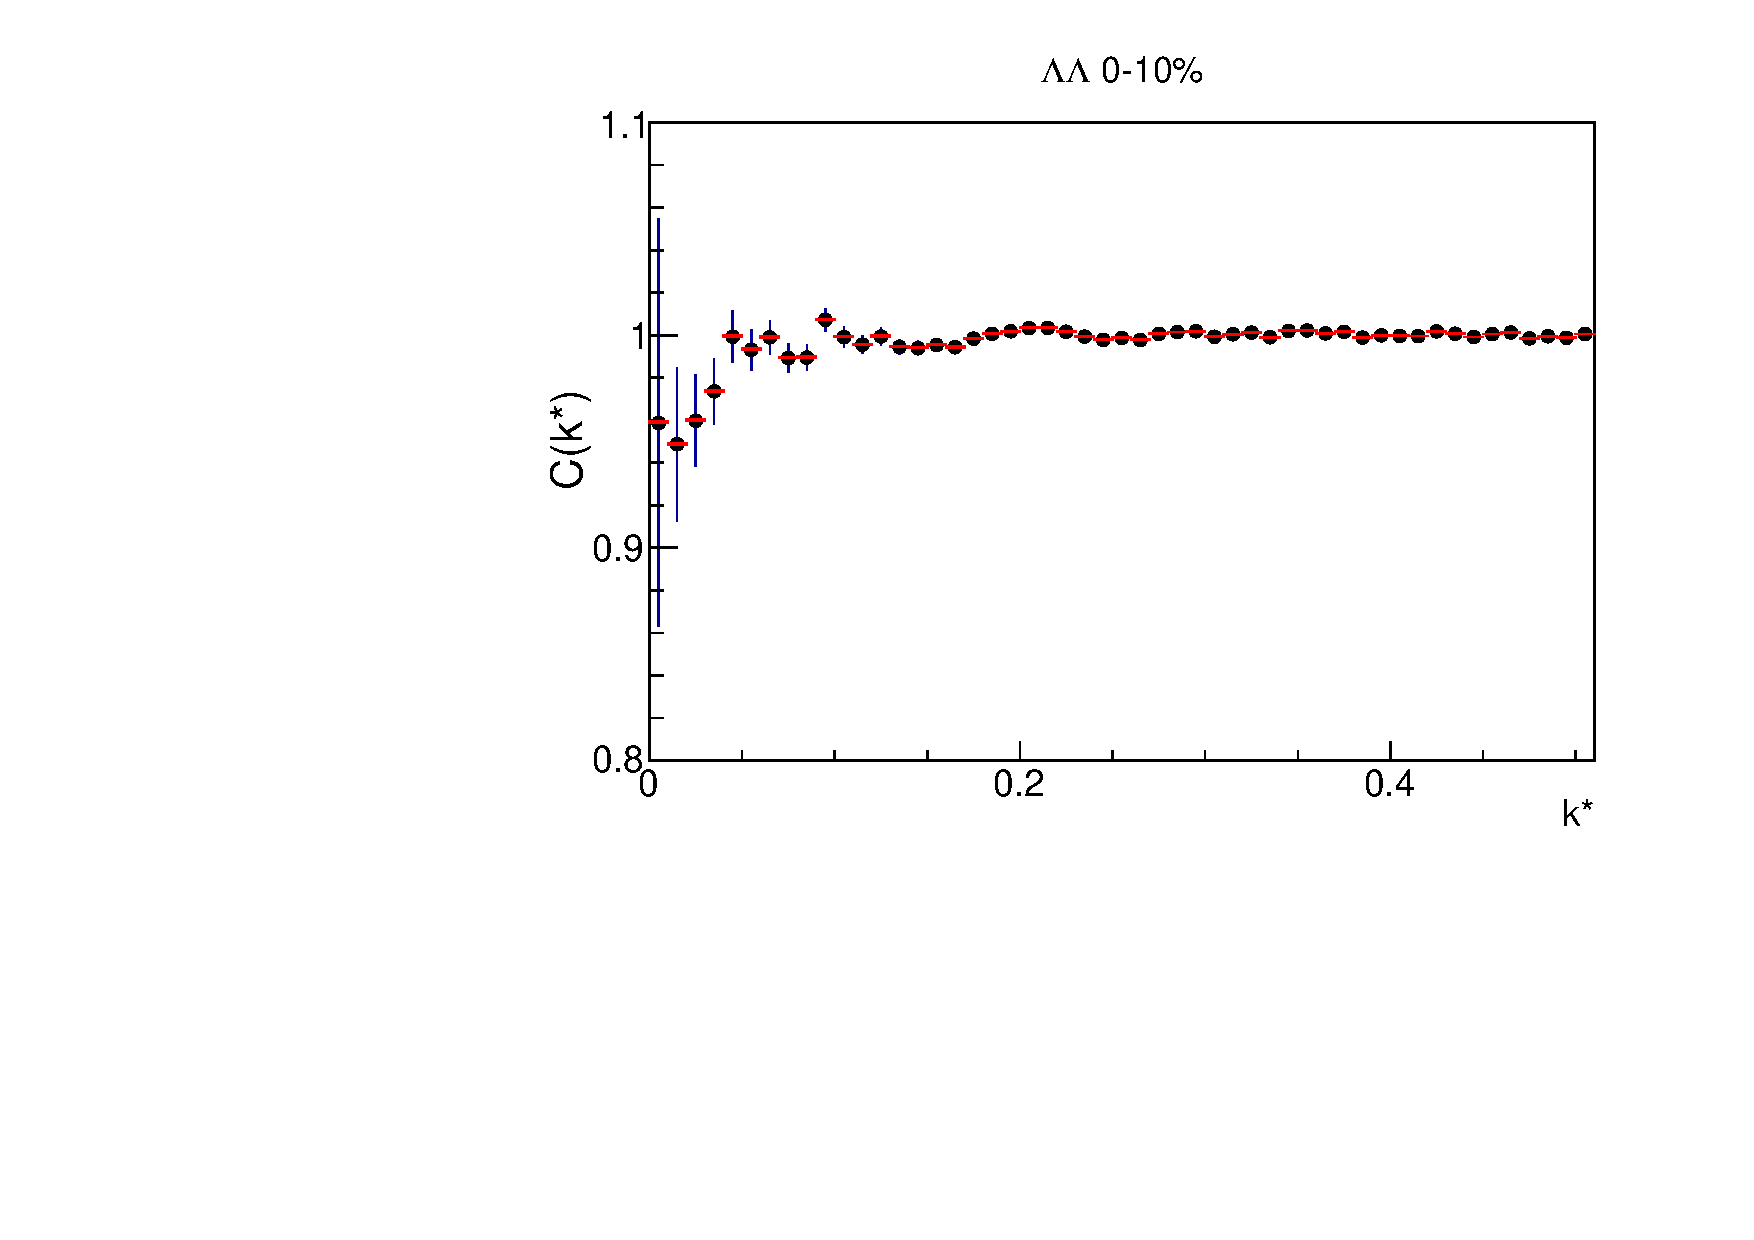
\includegraphics[width=36pc]{Figures/CFs/2016-8-30-CFLLAA010CombinedSystematicsMaximum.pdf}
\caption[$\Lambda\Lambda + \bar{\Lambda}\bar{\Lambda}$ correlation function for the 0-10\% centrality range]{$\Lambda\Lambda + \bar{\Lambda}\bar{\Lambda}$ correlation function for the 0-10\% centrality range with statistical and systematic errors.  
A dip at low $k^*$ is seen which is expected from quantum interference.}
\label{fig:CFLamLamALamALam010}
\end{figure}

\begin{figure}[hbt]
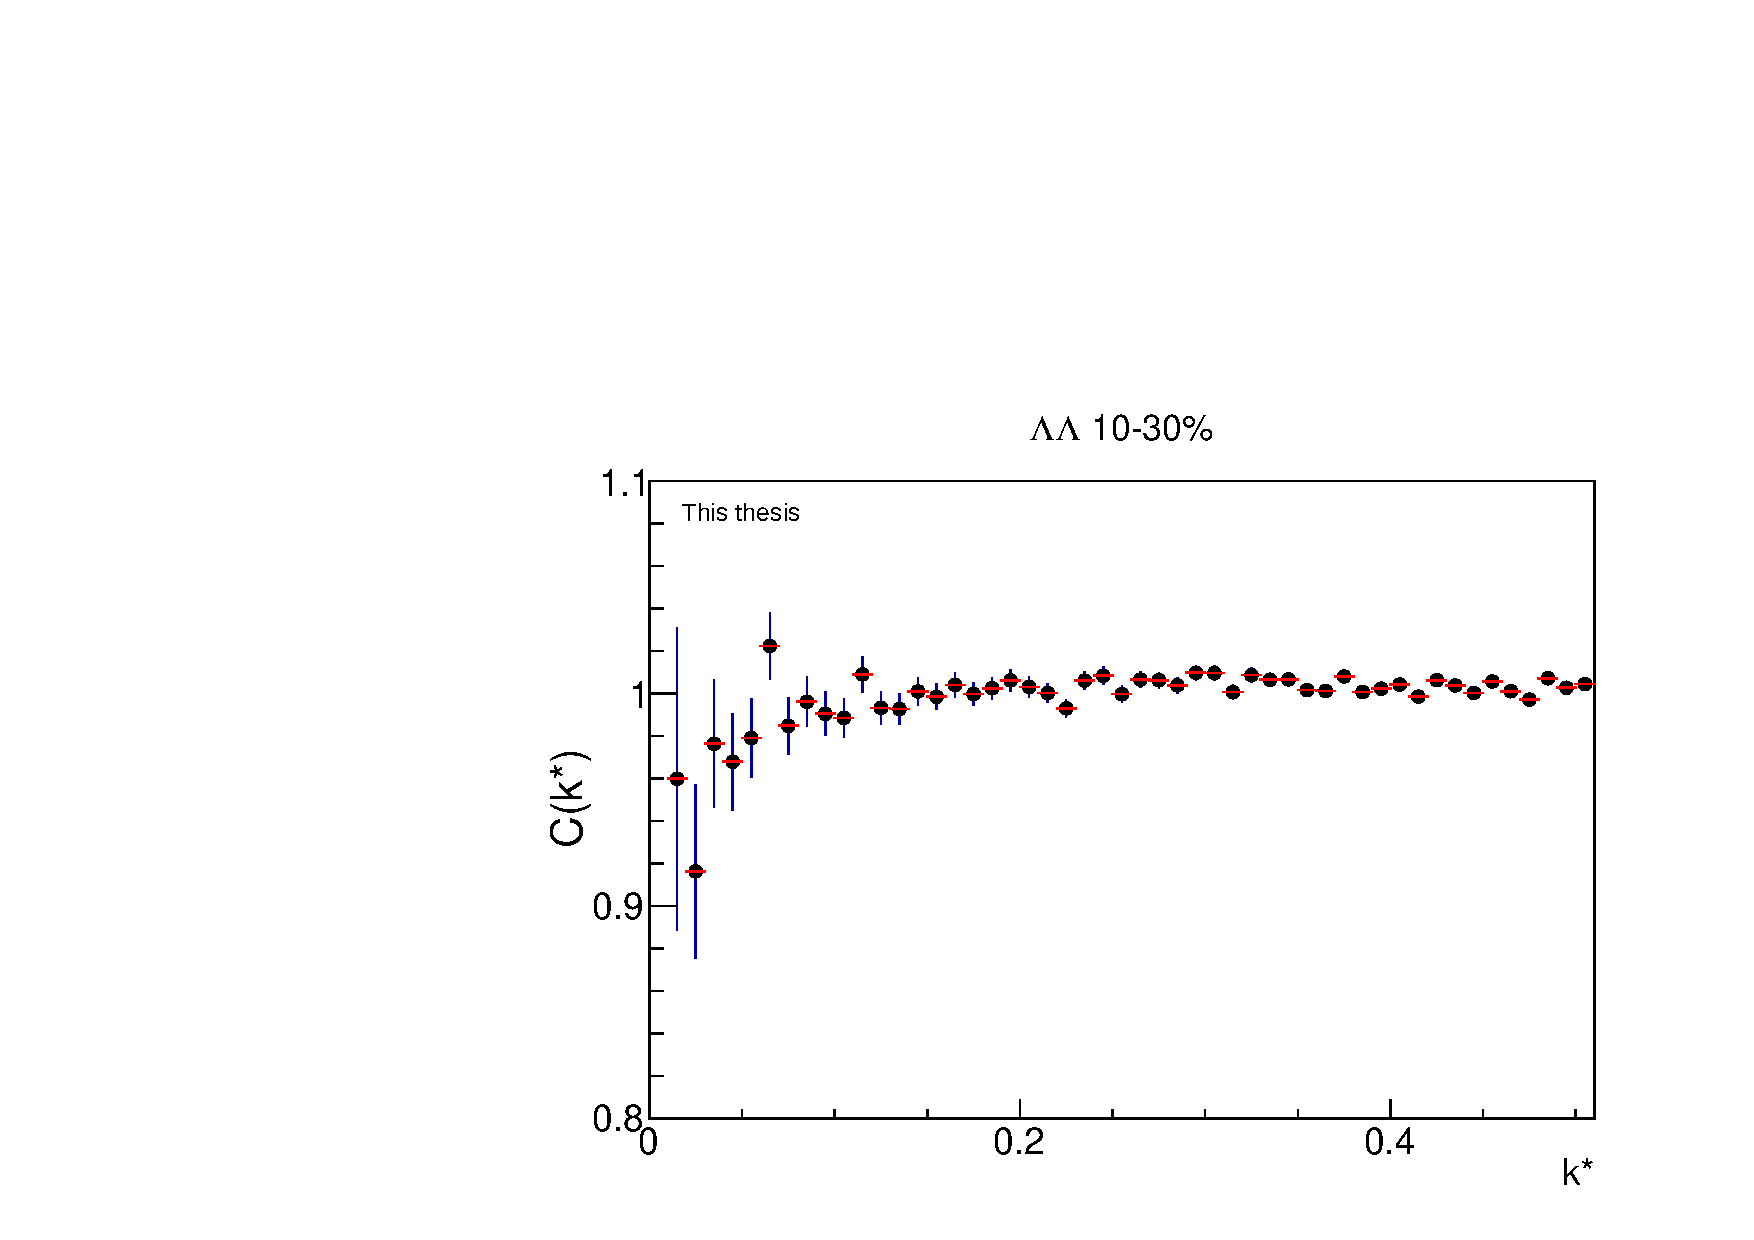
\includegraphics[width=36pc]{Figures/CFs/2016-8-30-CFLLAA1030CombinedSystematicsMaximum.pdf}
\caption[$\Lambda\Lambda + \bar{\Lambda}\bar{\Lambda}$ correlation function for the 10-30\% centrality range]{$\Lambda\Lambda + \bar{\Lambda}\bar{\Lambda}$ correlation function for the 10-30\% centrality range with statistical and systematic errors.  
A dip at low $k^*$ is seen which is expected from quantum interference.}
\label{fig:CFLamLamALamALam1030STAR}
\end{figure}

%\begin{figure}[hbt]
%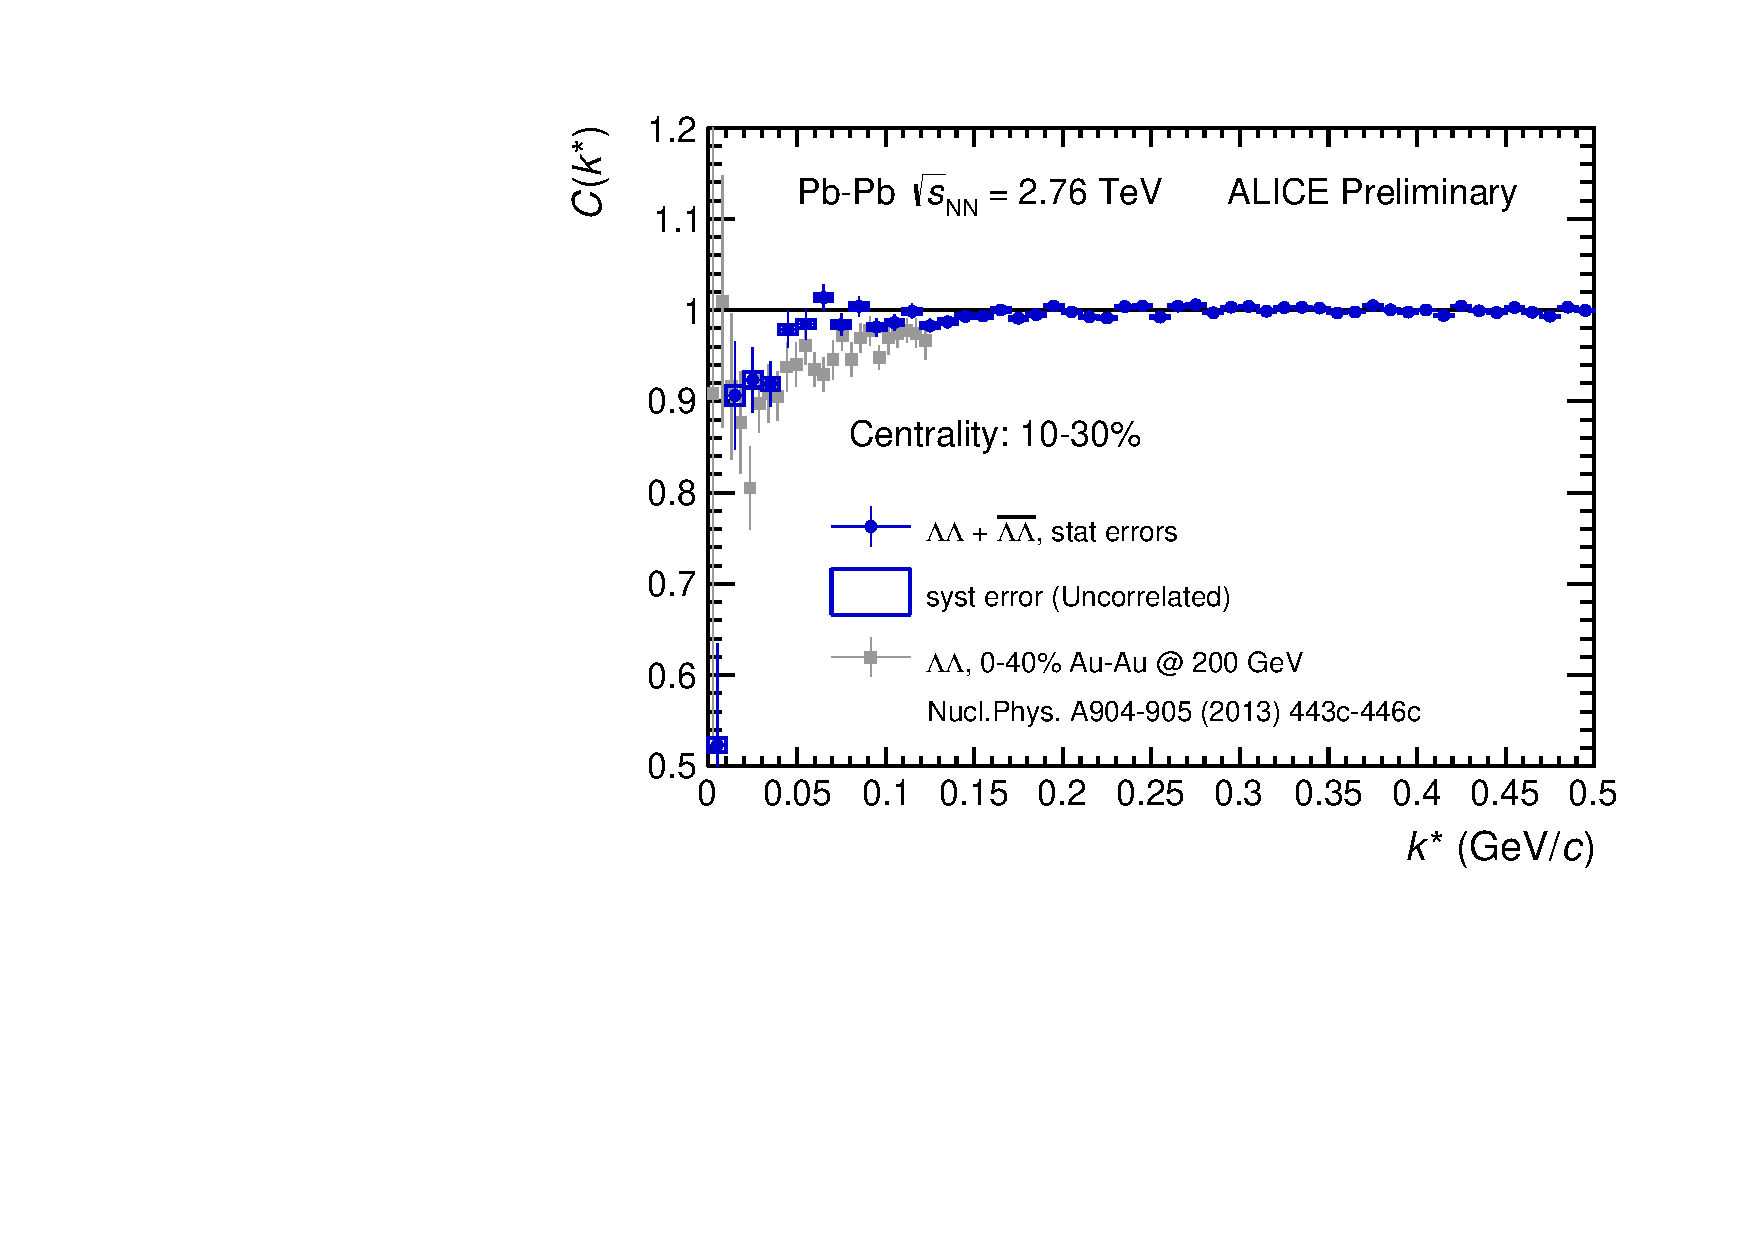
\includegraphics[width=36pc]{Figures/2014-05-11-CfLLAA-1030-CommentCorrections-WithSTAR.pdf}
%\caption[$\Lambda\Lambda + \bar{\Lambda}\bar{\Lambda}$ correlation function for the 10-30\% centrality range]{$\Lambda\Lambda + \bar{\Lambda}\bar{\Lambda}$ correlation function for the 10-30\% centrality range with statistical and systematic errors.  
%A dip at low $k^*$ is seen which is expected from quantum interference.  Preliminary STAR data for $\Lambda\Lambda$ is shown for comparison.  
%For the same plot without STAR data, see Figure \ref{fig:AppendixCFLamLamALamALam1030}.}
%\label{fig:CFLamLamALamALam1030STAR}
%\end{figure}

\begin{figure}[hbt]
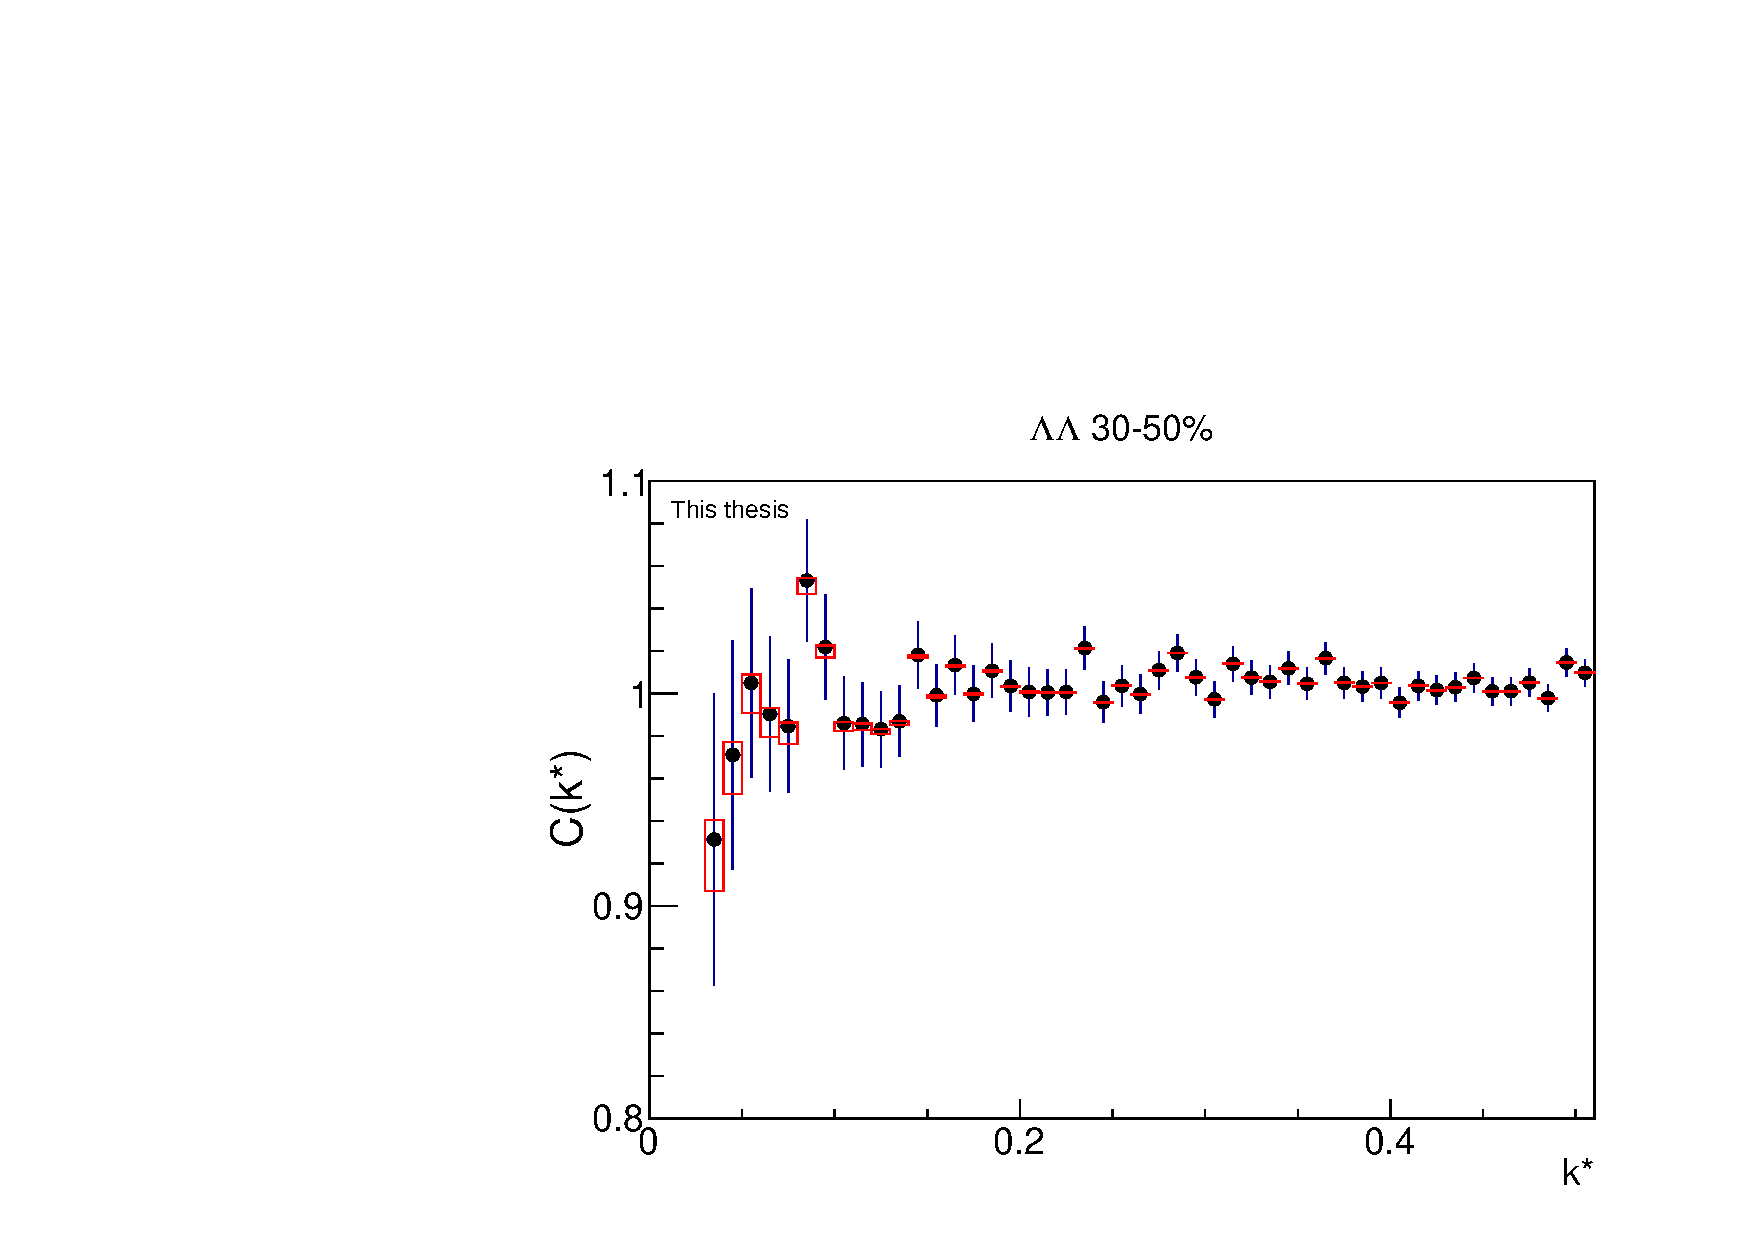
\includegraphics[width=36pc]{Figures/CFs/2016-8-30-CFLLAA3050CombinedSystematicsMaximum.pdf}
\caption[$\Lambda\Lambda + \bar{\Lambda}\bar{\Lambda}$ correlation function for the 30-50\% centrality range]{$\Lambda\Lambda + \bar{\Lambda}\bar{\Lambda}$ correlation function for the 30-50\% centrality range with statistical and systematic errors.  
Due to the poor statistics in the low $k^*$ region, it is not feasible to include this correlation function in the fit analysis.}
\label{fig:CFLamLamALamALam3050}
\end{figure}

\begin{figure}[hbt]
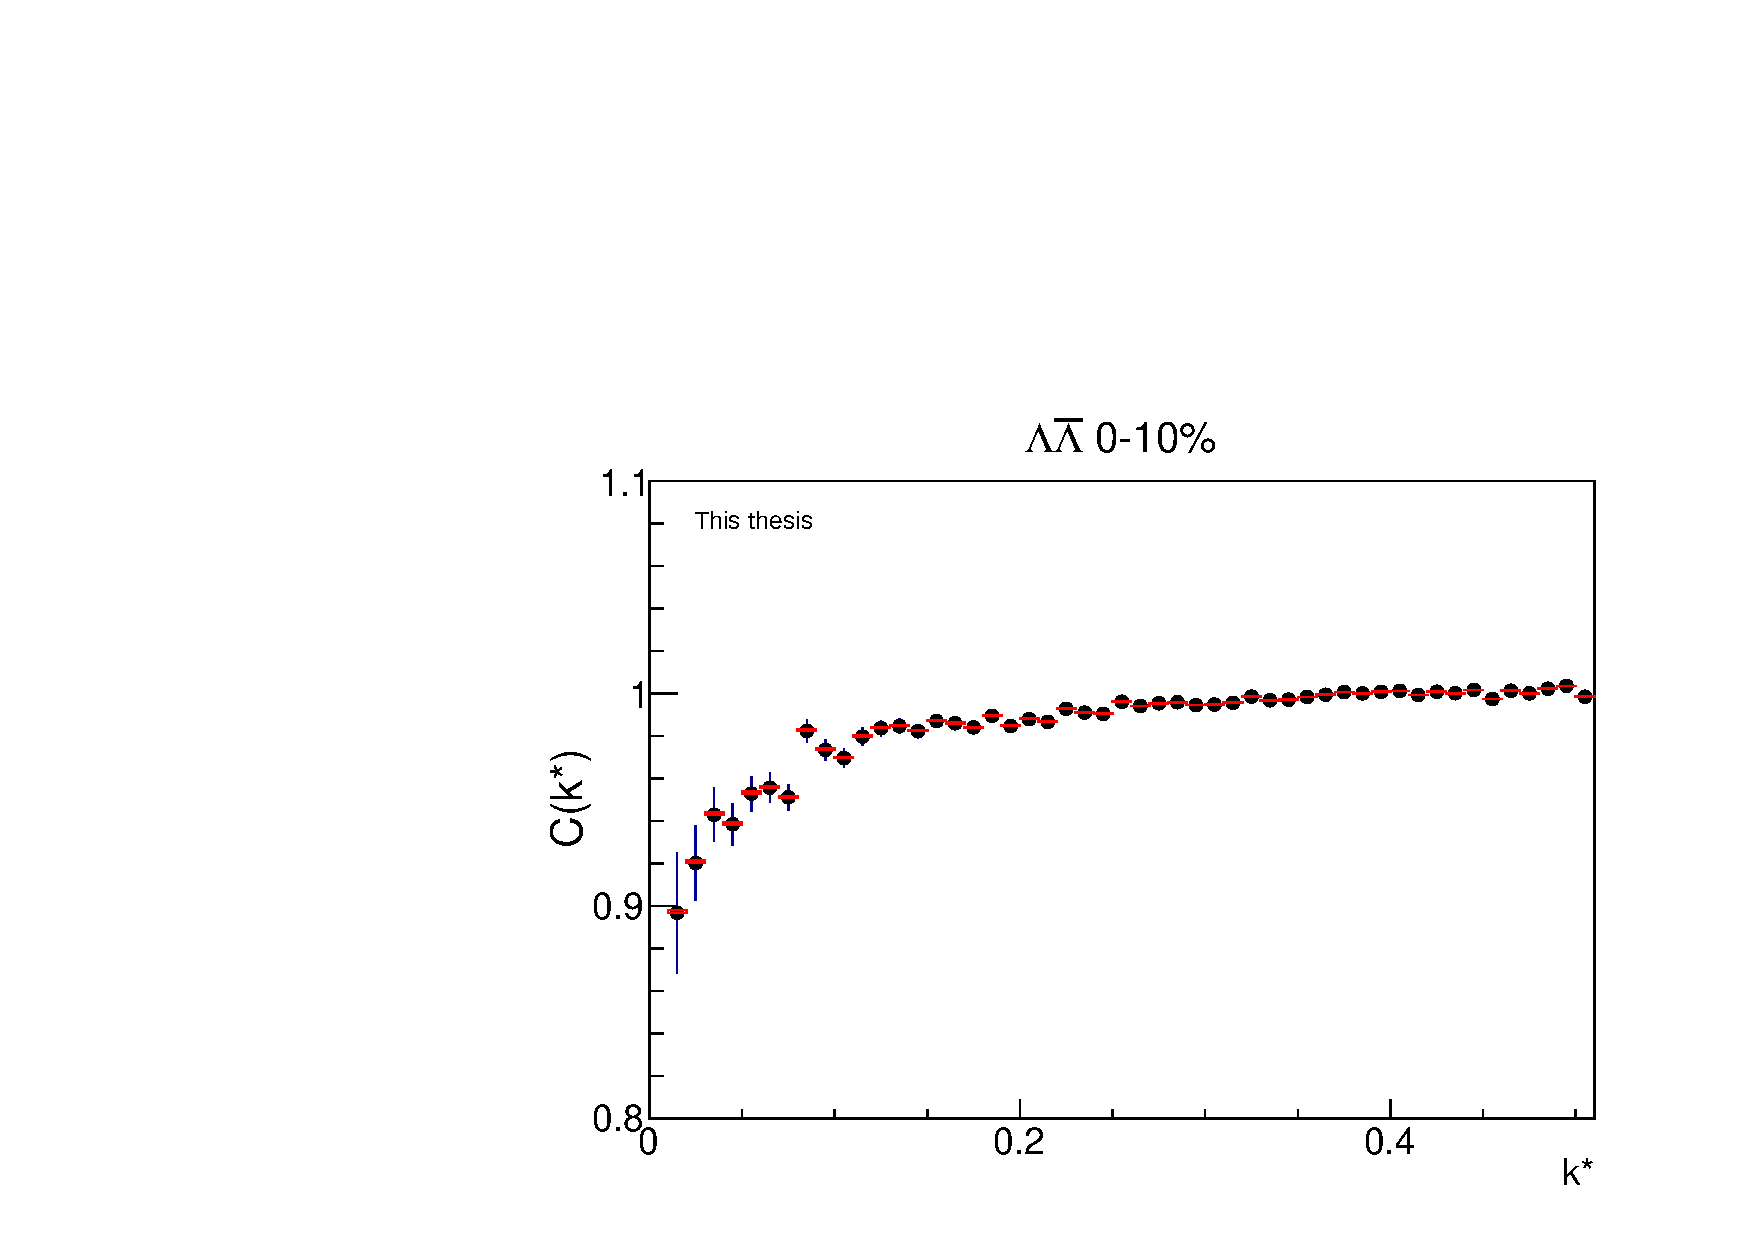
\includegraphics[width=36pc]{Figures/CFs/2016-8-30-CFLamALam010CombinedSystematicsMaximum.pdf}
\caption[$\Lambda\bar{\Lambda}$ correlation function for the 0-10\% centrality range]{$\Lambda\bar{\Lambda}$ correlation function for the 0-10\% centrality range with statistical and systematic errors.  
A wide suppression is seen which is indicative of annihilation.}
\label{fig:CFLamALam010}
\end{figure}
\begin{figure}[hbt]
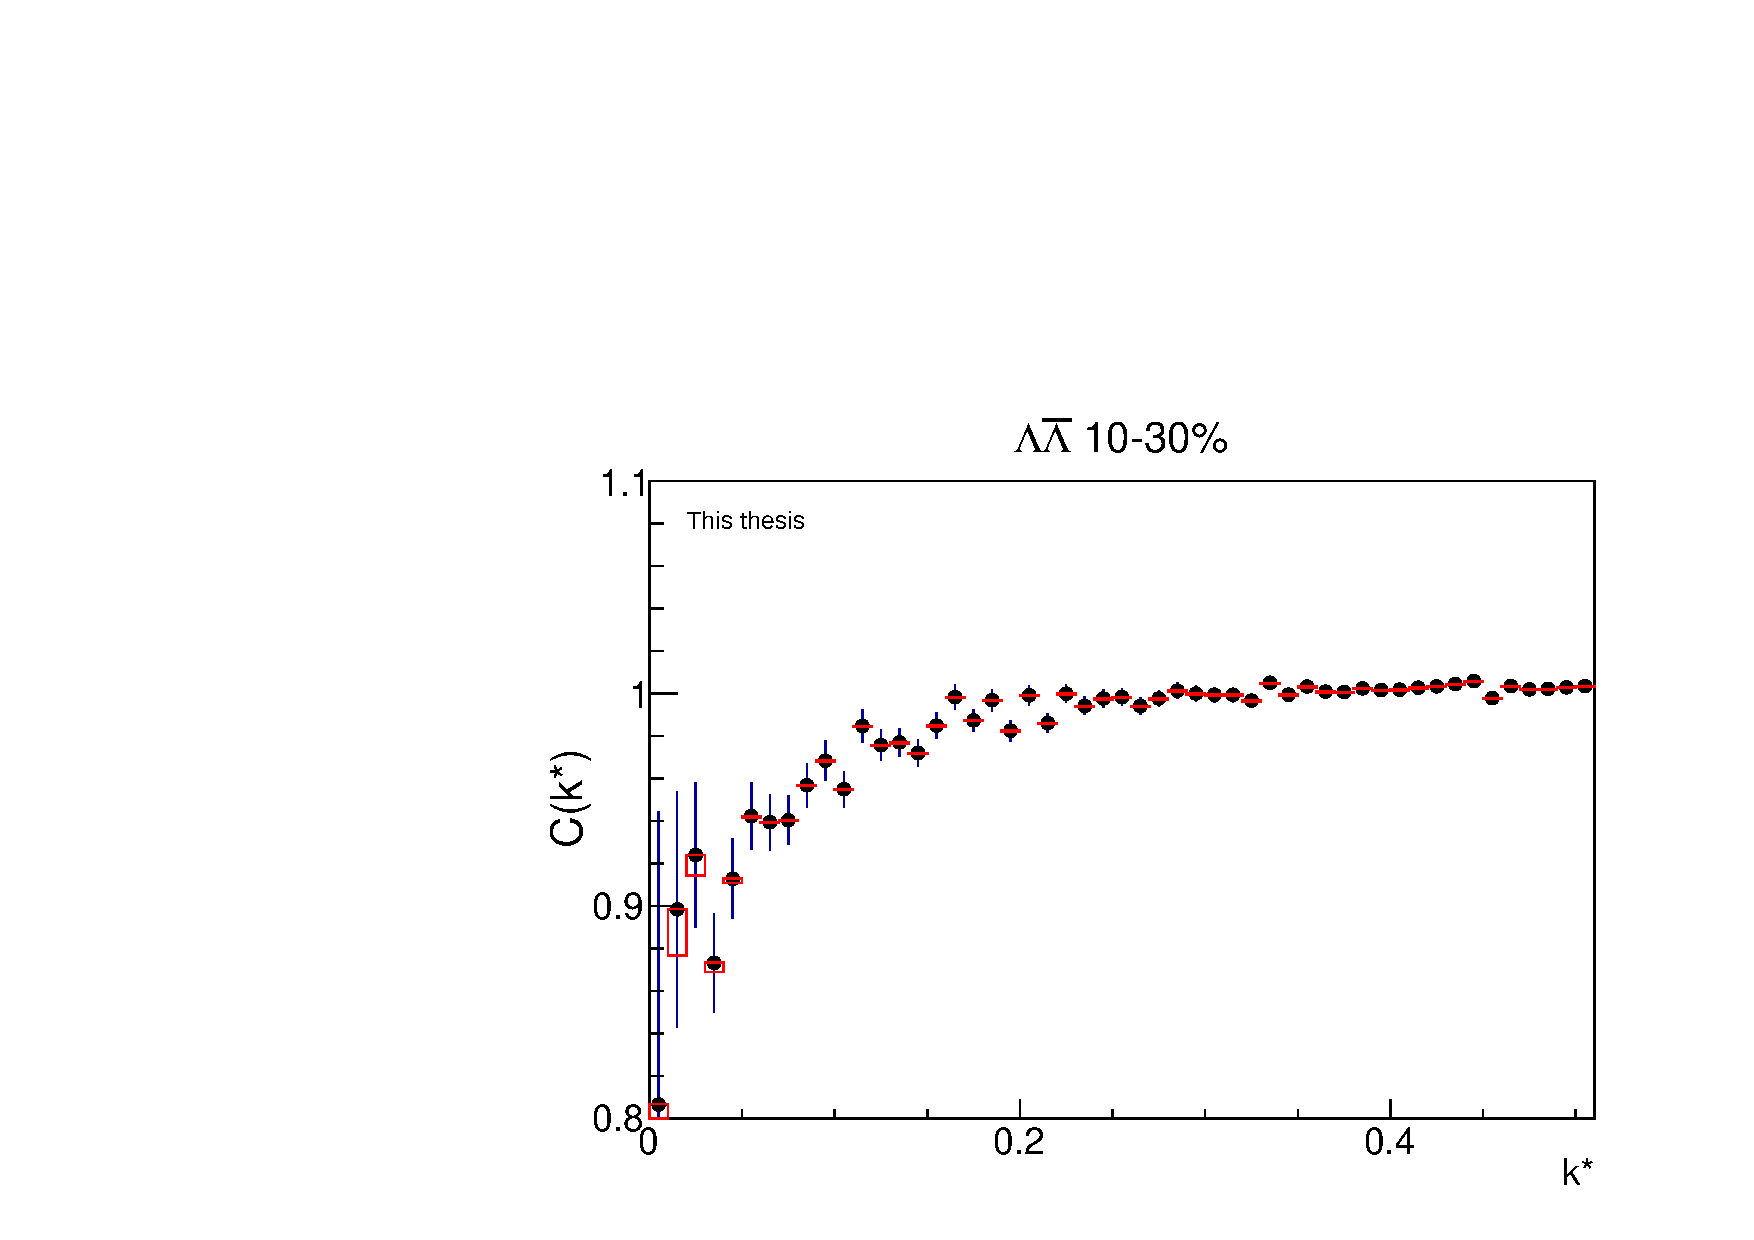
\includegraphics[width=36pc]{Figures/CFs/2016-8-30-CFLamALam1030CombinedSystematicsMaximum.pdf}
\caption[$\Lambda\bar{\Lambda}$ correlation function for the 10-30\% centrality range]{$\Lambda\bar{\Lambda}$ correlation function for the 10-30\% centrality range with statistical and systematic errors.  
A wide suppression is seen which is indicative of annihilation.}
\label{fig:CFLamALam1030}
\end{figure}
\begin{figure}[hbt]
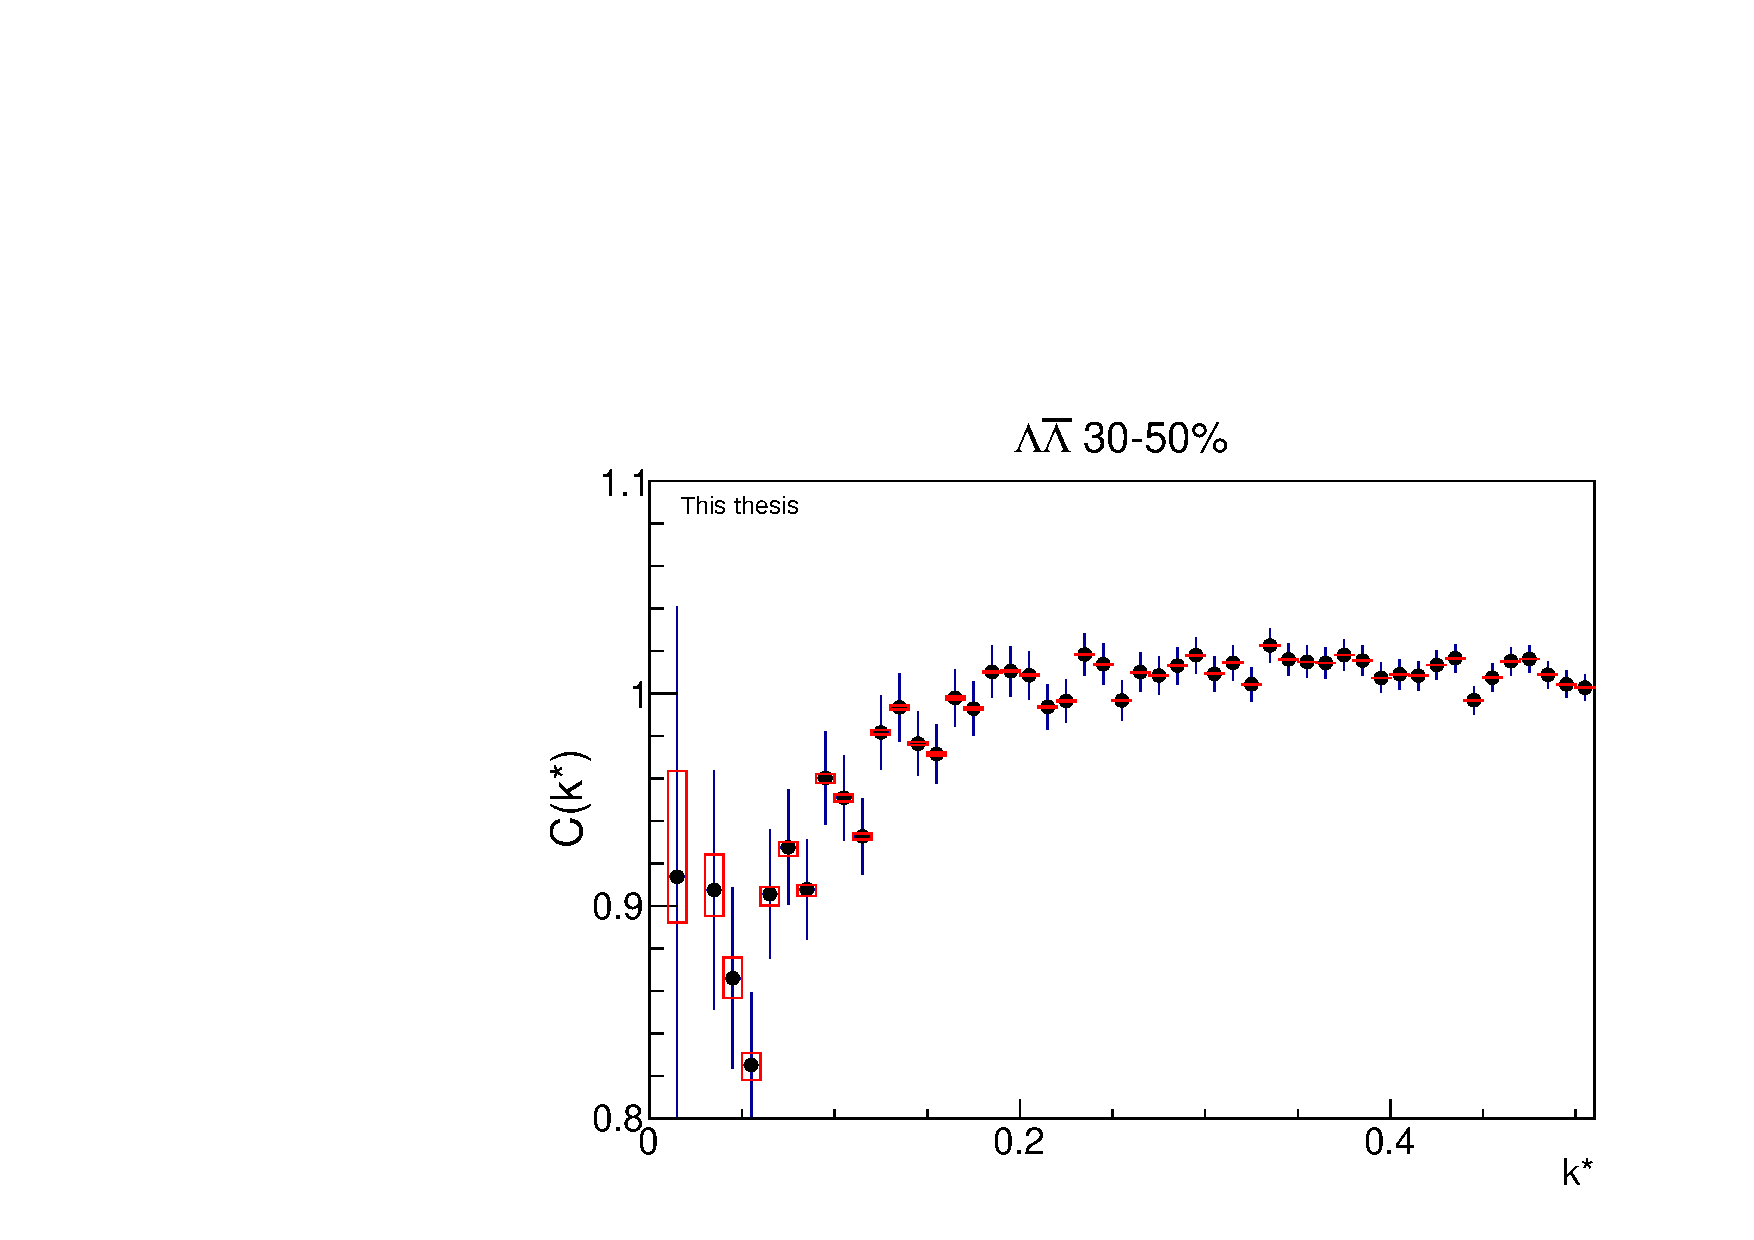
\includegraphics[width=36pc]{Figures/CFs/2016-8-30-CFLamALam3050CombinedSystematicsMaximum.pdf}
\caption[$\Lambda\bar{\Lambda}$ correlation function for the 30-50\% centrality range]{$\Lambda\bar{\Lambda}$ correlation function for the 30-50\% centrality range with statistical and systematic errors.  
A wide suppression is seen which is indicative of annihilation.}
\label{fig:CFLamALam3050}
\end{figure}

\begin{figure}[hbt]
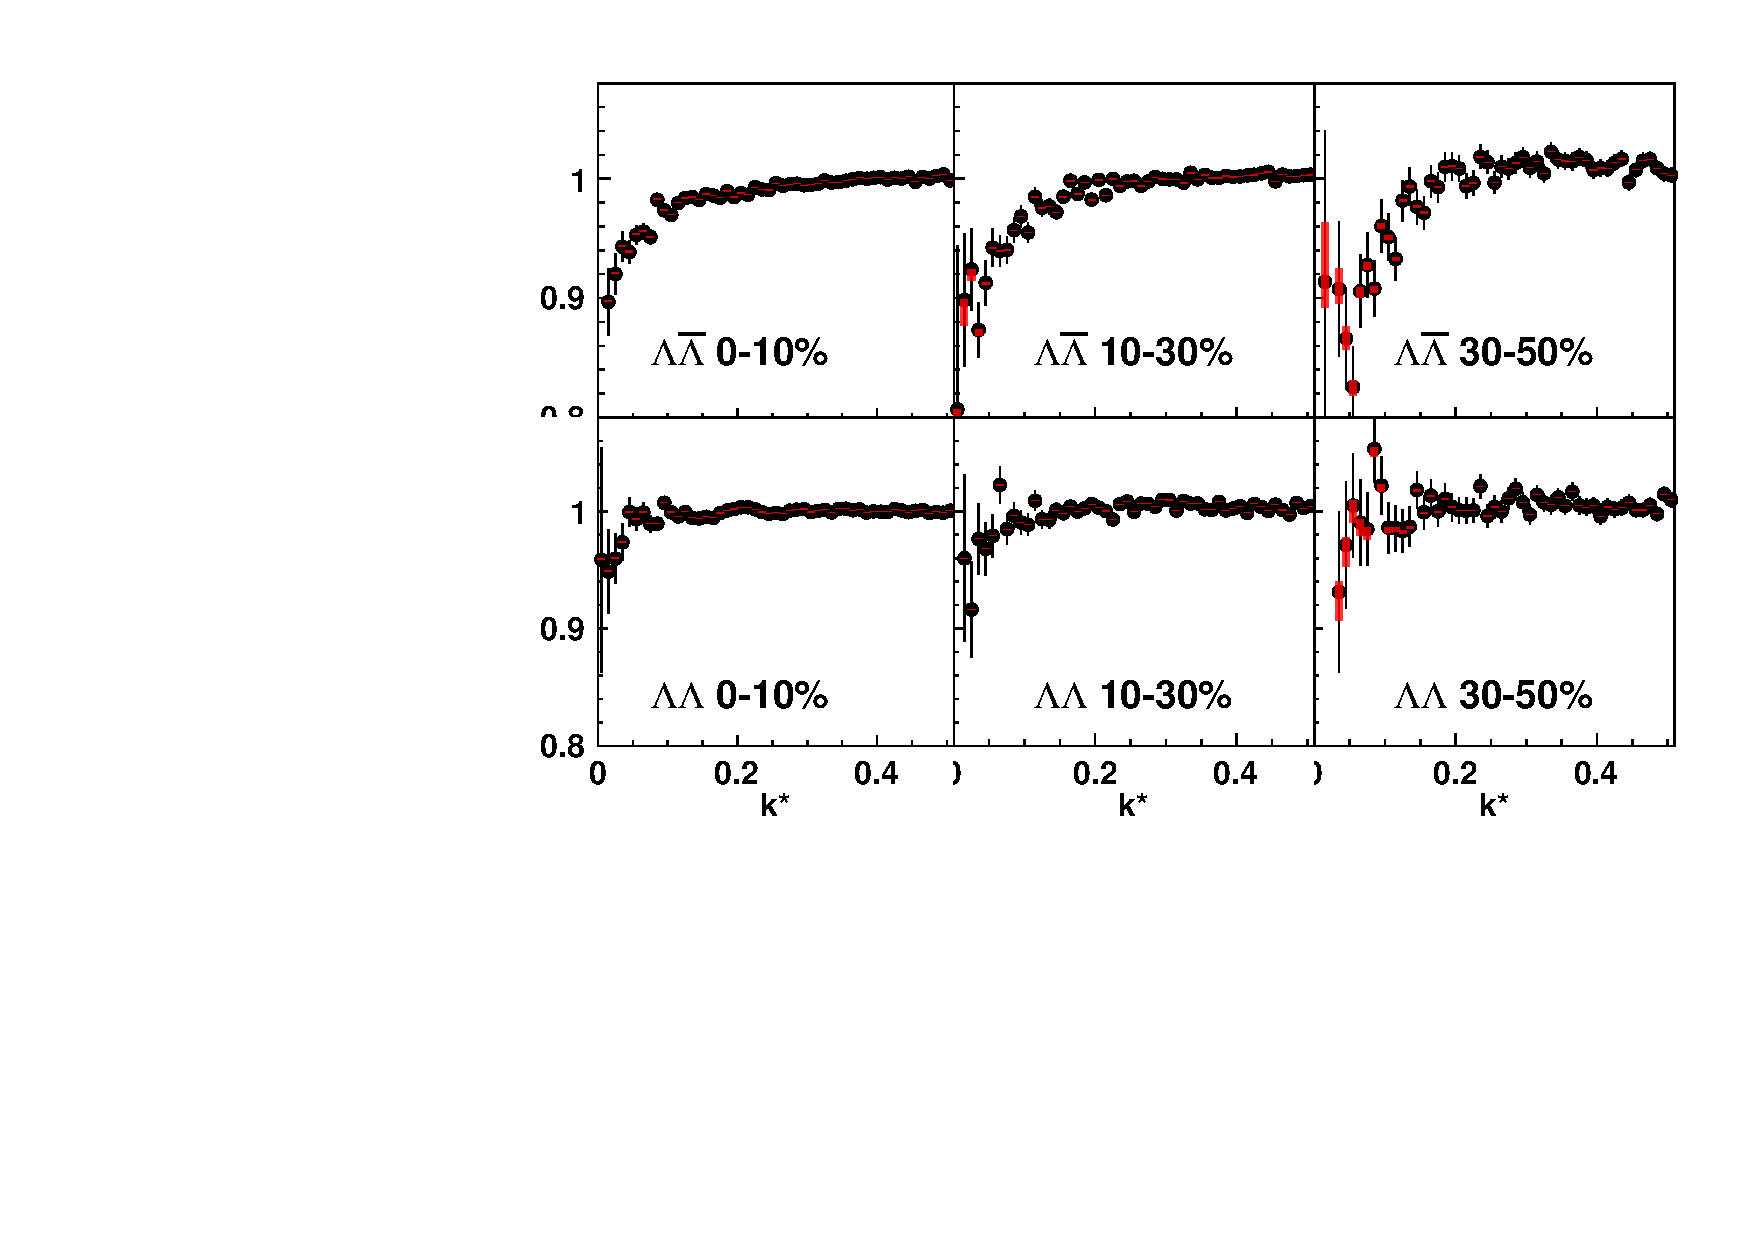
\includegraphics[width=36pc]{Figures/CFs/2016-08-30-AllCFsWithSysErrorsNoFit.pdf}
\caption[All $\Lambda\Lambda+\bar{\Lambda}\bar{\Lambda}$ and $\Lambda\bar{\Lambda}$ correlation functions]{$\Lambda\bar{\Lambda}$ (top) and $\Lambda\Lambda+\bar{\Lambda}\bar{\Lambda}$ (bottom) correlation functions for all three centrality ranges.}
\label{fig:CFAllOnOnePlot}
\end{figure}



\subsection{Interpretation of correlation function results}
\label{sec:CFInterpretation}


Generally speaking, the interesting part of a relative-momentum correlation function is the region below 100 or 200 MeV/c.  
Non-unity structures/backgrounds may be visible at large relative momentum - these structures can complicate the fitting procedure, and sometimes even direct attention to flaws in the analysis.  
They can also exist in the low-relative momentum region, though there they are generally assumed (or at least hoped) to be small.
However, the information about the source size and two-particle interactions is predominantly encoded within the low-$k^*$ region.  
For the time being, this analysis will restrict its attention to behavior in that region.
The non-femtoscopic background will be discussed more in Section \ref{sec:NonFemtoBackground}.

The $\Lambda\bar{\Lambda}$ correlation functions (Figures\ \ref{fig:CFLamALam010}, \ref{fig:CFLamALam1030}, and \ref{fig:CFLamALam3050}) exhibit a clear, centrality dependent suppression in the low-$k^*$ region, even with the significant statistical error bars for the 10-30\% and 30-50\% systems.  
A signal is also visible in the $\Lambda\Lambda + \bar{\Lambda}\bar{\Lambda}$ data, though it is smaller in magnitude and localized to a narrower $k^*$ region. 
%For reference, Preliminary STAR $\Lambda\Lambda$ results from 200 GeV Au--Au, 0-40\% centrality are also plotted \cite{Shah:2012ps}.

Several factors may contribute to the small size of this signal.  
First of all, the physics of the identical particle systems (see Sec.\ \ref{sec:AnalyticModel}) is expected to be confined to just the few lowest bins.  
There may be competing physics effects -- a suppression from quantum interference and an enhancement from the strong final state interactions -- that wash each other out.  
Furthermore, two-track effects like splitting and merging show up in this region, though they are assumed to be well-corrected for by the aforementioned pair-wise cuts.  
The presence of residual correlations may also muddle or dilute the signal region.  
This will be discussed further in Section \ref{sec:Residual}.  
%Finally, it must be noted that these are the $k^*$ bins with the least statistics.  
%There are also a couple of fitting tricks that can be employed to mitigate the statistical limitations in these plots.  
%They will be discussed in Section \ref{sec:MinuitFit}.

%********Outdated****** some of this may be salvageable

%Figure \ref{fig:CFMixCentralities} shows $\Lambda\bar{\Lambda}$ correlation functions versus $q_{\rm inv}$ for three different centralities ranges.  The correlations are normalized to unity in the $ 0.3 < q_{\rm_{inv}} < 0.5$ GeV/c range.  Each correlation shows clear suppression in the low-$q_{\rm_{inv}}$ region, which is considered an effect of the baryon-antibaryon annihilation channel.  The strength of the correlation effect increases with more peripheral events, an indication that the emitting source size is shrinking for those events.

%Figure \ref{fig:CF} shows correlation functions constructed in the 0-10\% centrality range for $\Lambda\Lambda$ and $\bar{\Lambda}\bar{\Lambda}$ pairs.  Both correlation functions exhibit an enhancement in the low-$q_{\rm inv}$ range of 0.04 - 0.2 GeV/c.  This may be due to attractive final state interactions.  The effects of FSI and quantum statistics are expected to be seen in roughly the same $q_{\rm inv}$ range, and it is unclear at this time to what extent their effects should be competing. The enhancement of the $\bar{\Lambda}\bar{\Lambda}$ correlation function does fall off in the lowest bins, though the statistical uncertainties are such that no significant statement about the effects of quantum statistics can be made at this time.



